\chapter{Richiami teorici}
\section{Teoria della similitudine}
L’applicazione della teoria della similitudine costituisce un primo e potente strumento della progettazione, in particolar modo per quanto riguarda le turbomacchine. La teoria della similitudine permette di risolvere diversi problemi:
\begin{itemize}
\item[$-$] note le prestazioni di una macchina che ha determinate dimensioni, si possono ricavare le prestazioni di una macchina geometricamente simile a quella considerata ma di diverse dimensioni nel dettaglio; questo permette la realizzazione di prototipi in scala ridotta. Un esempio tipico: modellino della grande turbina idraulica che viene provato prima di procedere alla costruzione della macchina vera;
\item[$-$] nota una ben determinata condizione di funzionamento di una turbomacchina, come potrebbero essere le condizioni di progetto, si possono individuare altre condizioni di funzionamento ottenute variando la velocità di rotazione, la portata, oppure il lavoro scambiato (fluido/macchina);
\item[$-$] curve di prestazioni rilevate in determinate condizioni ambientali possono essere espresse in funzione di parametri che sono invarianti al variare delle condizioni ambientali stesse. In questo modo è possibile conoscere le prestazioni di una macchina operante in condizioni diverse (ad esempio un compressore al livello del mare ad agosto e in montagna a Natale);
\item[$-$]si può stabilire in maniera semplice e veloce fin da subito quale sarà il tipo di macchina migliore da usare, quale sarà la sua geometria di base e quali le dimensioni generali; questo si rivela essere un ausilio al designer in sede di progettazione. Grazie a ciò si riesce a sfruttare l’esperienza già maturata nella progettazione, sviluppo e test di altre macchine simili. Perciò, possedere un database ricco di informazioni relative a macchine pregresse, risulta essere un vantaggio progettuale non di poco conto.
\end{itemize}

ll teorema di Buckingham (conosciuto anche come teorema $\pi$), dovuto al fisico statunitense Edgar Buckingham, afferma:
\begin{quotation}
	Dato un problema descritto da un certo numero di equazioni in cui siano presenti $n$ variabili fisiche, se le dimensioni fondamentali di queste variabili sono $x$ allora il problema può essere completamente descritto da $n - x$ variabili adimensionali.
\end{quotation}
Per studiare il comportamento di una turbomacchina si definisce il seguente funzionale.
\begin{equation}
f(D_i,l_j,\dot{m},w,L_i,\mu,a_{01},\rho_{01})=0
\end{equation}
con:\\[1mm]
$D_i$: serie di diametri rilevanti;\\
$l_j$: serie di lunghezze rilevanti;\\
$\dot{m}$: portata in massa;\\
$w$: velocità angolare;\\
$L_i$: lavoro ideale scambiato tra macchina e fluido per unità di massa;\\
$\mu$: viscosità dinamica del fluido;\\
$a_{01}$: velocità del suono all'ingresso in condizioni di ristagno;\\
$\rho_{01}$: densità del fluido.\\[2mm]
Si definiscono poi il numero di Reyonlds e il numero di Mach:
\begin{equation}
Re= \frac{\rho_{01} w D^2}{\mu}
\end{equation}
\begin{equation}
Ma= \frac{w D}{a_{01}}
\end{equation}
Si evidenzia che tutti gli argomenti del funzionale sono descritti da una combinazione delle tre grandezze fondamentali [M] [L] [T], ovvero massa lunghezza e tempo. Tenendo presente ciò è possibile adimensionalizzare gli argomenti del funzionale ottenendo una nuova espressione per lo stesso.\\
In una macchina termica in cui le proprietà del fluido cambiano nei vari punti della macchina, per definire la densità o la velocità del suono bisogna fissare convenzionalmente una condizione rispetto alla quale vado a valutare quella proprietà.
Una condizione di riferimento che viene spesso adottata (non è l’unica) è quella di valutare queste quantità nelle condizioni totali all’ingresso della macchina (cioè condizioni valutate immaginando il fluido in quiete) che possiamo indicare con il pedice $01$ ($0$: condizioni totali o di ristagno; $1$: condizioni di ingresso).\\
Si può allo stesso modo definire le cifre di flusso $\varphi$ e di pressione $\psi$ andando ad adimensionalizzare rispettivamente la portata e il lavoro unitario:
\begin{equation}
\varphi = \frac{\dot{m}}{\rho_{01}w D^3} \left( =\frac{Q}{w D^3} \right)
\end{equation}
\begin{equation}\label{eq:psi}
\psi = \frac{L_i}{w^2 D^2}
\end{equation}
Il funzionale può essere espresso quindi secondo i numeri adimensionali:
\begin{equation}
f(\pi_i,\pi_j,\varphi,\psi,Re,Ma)=0
\end{equation}
Supponendo di confrontare due macchine, se queste hanno le gli stessi valori di $\pi_i$ e $\pi_j$, allora la geometria tra le due macchine può da considerarsi simile e sotto queste ipotesi il funzionale si semplifica:
\begin{equation}
f(\varphi,\psi,Re,Ma)=0
\end{equation}
\begin{figure}
\centering
  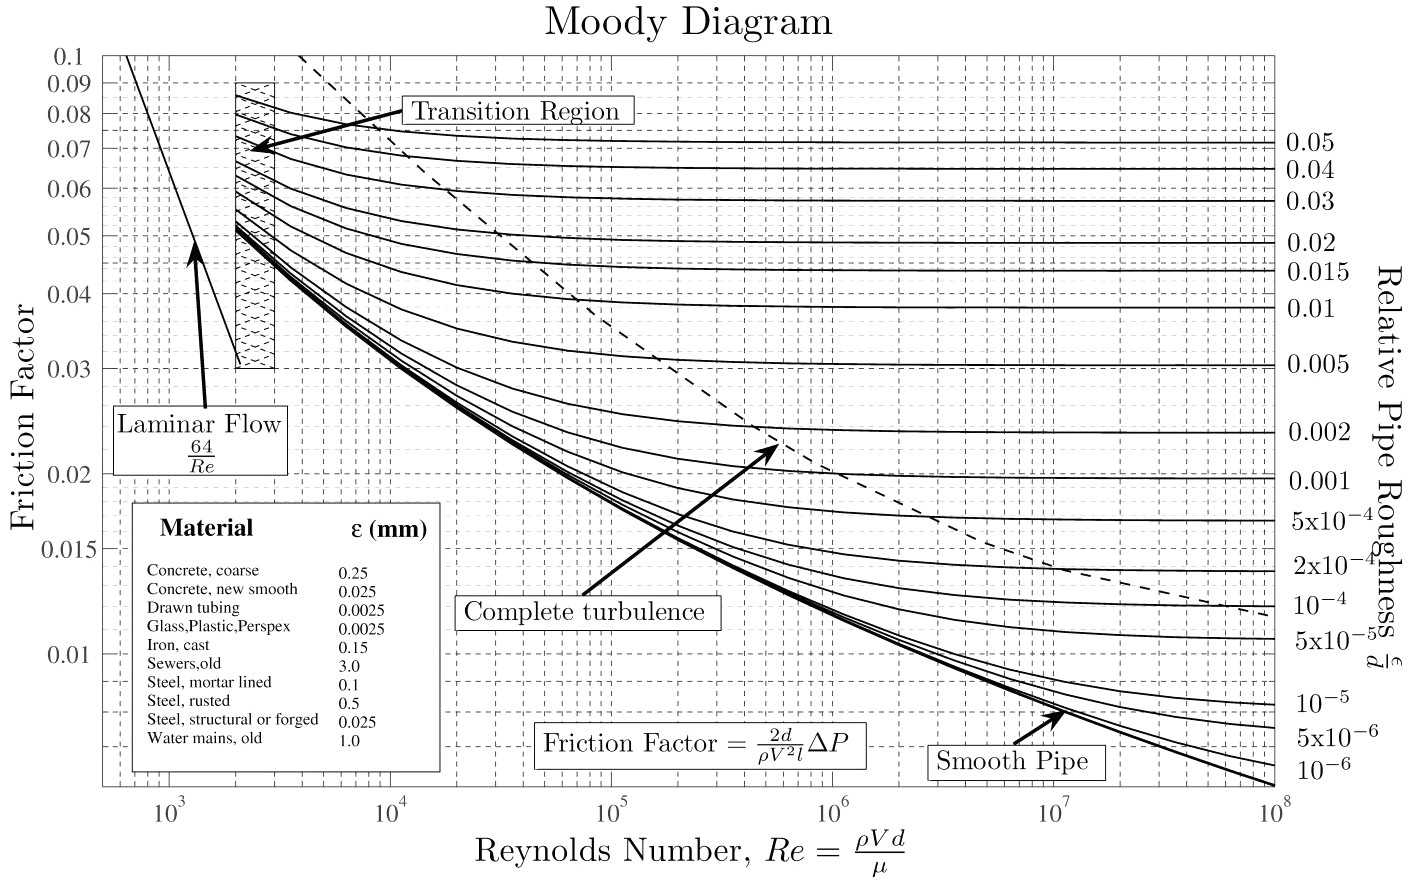
\includegraphics[width=\textwidth]{fig/moody.jpg}
\caption{}
\label{fig:moody}
\end{figure}
Guardando il diagramma di Moody in figura \ref{fig:moody}, sull'asse delle ascisse è presente $Re$ ed su quello delle ordinate il coefficiente di perdita di carico del nostro tubo $\xi$. Le scale sono logaritmiche. Il legame tra $\xi$ e $Re$, per bassi numeri di Reynolds, è rappresentato da una retta. Poi si ha una zona di transizione non ben definita ed infine una serie di linee a rugosità relativa costante $\epsilon/D$ (con $\epsilon$ rugosità media).\\
Nel primo tratto di legame lineare si ha una corrente laminare. Il tratto tratteggiato è un tratto nel quale, in condizioni sperimentali assolutamente controllate, è possibile mantenere un flusso laminare ma altamente instabile. In condizioni di flusso turbolento la perdita di carico dipende dalla rugosità.\\
\'E possibile inoltre osservare che se si considera un solo valore di rugosità relativa, la curva presenta una certa pendenza fino ad un certo valore di $Re$ (limite o critico) per poi diventare orizzontale. Sotto le ipotesi di moto turbolento pienamente sviluppato si trascura l’influenza di Reynolds nel funzionale. Va ovviamente considerato che le rugosità relative di una macchina grande saranno in genere diverse da quelle che si possono ottenere con macchine piccole.\\
Quindi se il numero di Reynolds è superiore ad un certo valore limite, il coefficiente di perdita di carico è indipendente da $Re$. Trasferendo questa osservazione alla turbomacchina si può verificare sperimentalmente che se $Re$ è molto elevato questo potrà anche variare ma le prestazioni non ne saranno influenzate. Perciò il funzionale si semplifica ulteriormente in:
\begin{equation}
f(\varphi,\psi,Ma)=0
\end{equation}
In seguito, si aggiungerà una perdita sul modello in quanto il rendimento di una macchina piccola sarà sempre inferiore al rendimento di una macchina grande.\\
In ultimo, se si trascurano i fenomeni di comprimibilità si può trascurare anche il numero di Mach; equivalentemente si fa l'ipotesi $Ma<0.3$. Perciò il funzionale risulta:
\begin{align*}
f(\varphi,\psi)=0
\end{align*}
Dotando la pompa di un sensore per la rilevazione di pressione, numero di giri e portata, è possibile andare a definire una curva di prestazione adimensionale.

Si definiscono le tre componenti del vettore velocità:
\begin{itemize}
\item[$c$]: velocità assoluta;
\item[$w$]: velocità relativa;
\item[$u$]: velocità periferica;
\end{itemize}
Naturalmente affinché le macchine operino in condizioni di similitudine devono, per definizione, avere $\varphi$ e $\psi$ uguali. Vale inoltre le seguenti relazioni tra cifre di flusso e di pressione e le componenti dei triangoli di velocità:
\begin{equation}
\varphi=\frac{Q}{w D^3} \propto \frac{c_m}{u}
\end{equation}
\begin{equation}
\psi = \frac{L_i}{w^2 D^2} \propto \frac{c_u}{u}
\end{equation}
con $u= \omega \times r$. Perciò mantenere $\varphi$ e $\psi$ uguali significa avere triangoli di velocità simili (vedi la figura \ref{fig:tria}).
\begin{figure}
\centering
  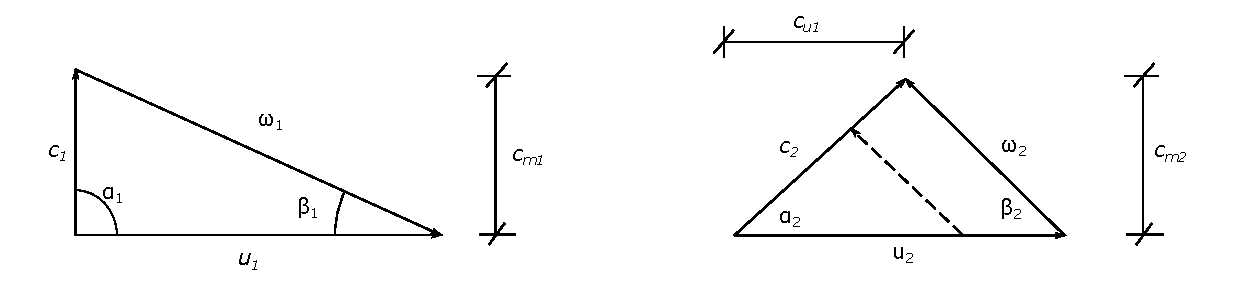
\includegraphics[width=.8\textwidth]{fig/triang.pdf}
\caption{Triangoli di velocità in ingresso e in uscita per una macchina radiale centrifuga "elementare"}
\label{fig:tria}
\end{figure}

Si considera ora il caso di una macchina idraulica e si cerca il luogo dei punti di funzionamento simili sul piano delle prestazioni; questo permette di capire come le curve delle prestazioni adimensionali stiano in rapporto con le curve delle prestazioni dimensionali.\\
Rilevando le prestazioni di una pompa si ottiene la curva di funzionamento caratteristica (diagramma prevalenza - portata) per un certo valore della velocità di rotazione (figura \ref{fig:hq}).
\begin{figure}[h!]
\centering
  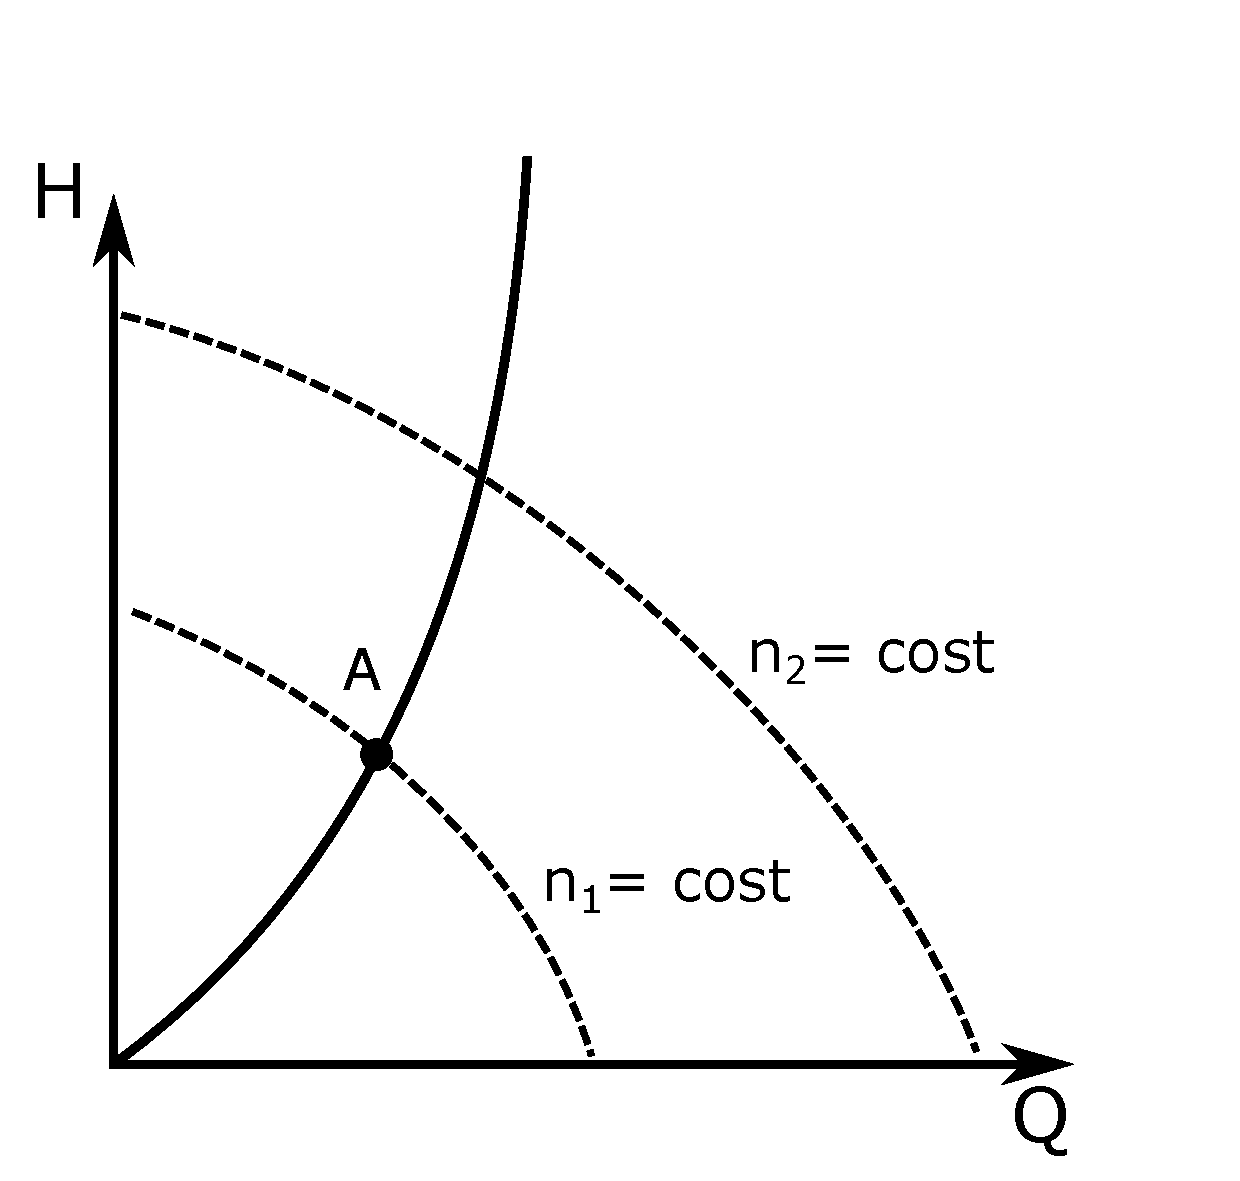
\includegraphics[width=.3\textwidth]{fig/hq.pdf}
\caption{}
\label{fig:hq}
\end{figure}
Queste curve sono espresse in funzione di grandezze dimensionali, ma andando ad adimensionalizzarle si possono ottenere tali curve in funzione delle relative cifre di pressione e di flusso.\\
Si consideri una condizione di funzionamento $A$: il luogo dei punti di funzionamento simili ad $A$ sarà caratterizzato dal fatto di avere stessi $\varphi$ e $\psi$. Considerando quindi il generico punto $x$ si può scrivere:
\begin{equation}
\varphi = \frac{Q}{w D^3}= \frac{Q_x}{w_x D^3}
\end{equation}
Per una macchina con lo stesso diametro si può scrivere:
\begin{equation}
\frac{Q_x}{Q}=\frac{w_x}{w} \;\;\;\; \Rightarrow \;\;\;\; Q_x = Q \frac{w_x}{w}
\end{equation}
Imponendo l'uguaglianza della cifra di pressione ($L_i=gH$ perché si sta considerando una macchina idraulica):
\begin{equation}
\psi = \frac{gH}{w^2 D^2}= \frac{gH_x}{w_x^2 D^2}
\end{equation}
In questo modo si ottiene:
\begin{equation}
H_x = H\bigg(\frac{w_x}{w}\bigg)^2 = H\bigg(\frac{Q_x}{Q}\bigg)^2 \;\;\;\; \Rightarrow \;\;\;\; H_x = \frac{H}{Q^2}Q_x^2
\end{equation}
che è l'equazione di una parabola sul piano H - Q, passante per il punto A e per l'origine degli assi. Il lavoro varia con il quadrato della velocità angolare mentre la portata varia linearmente rispetto la velocità angolare.

Ad ogni curva $\varphi - \psi$ corrisponde una curva di rendimento; si può quindi individuare una coppia di valori $\bar{\varphi} - \bar{\psi}$ ottimali in cui il rendimento è massimo (figura \ref{fig:adim}) e definire il coefficiente di velocità periferica:
\begin{figure}[h!]
\centering
  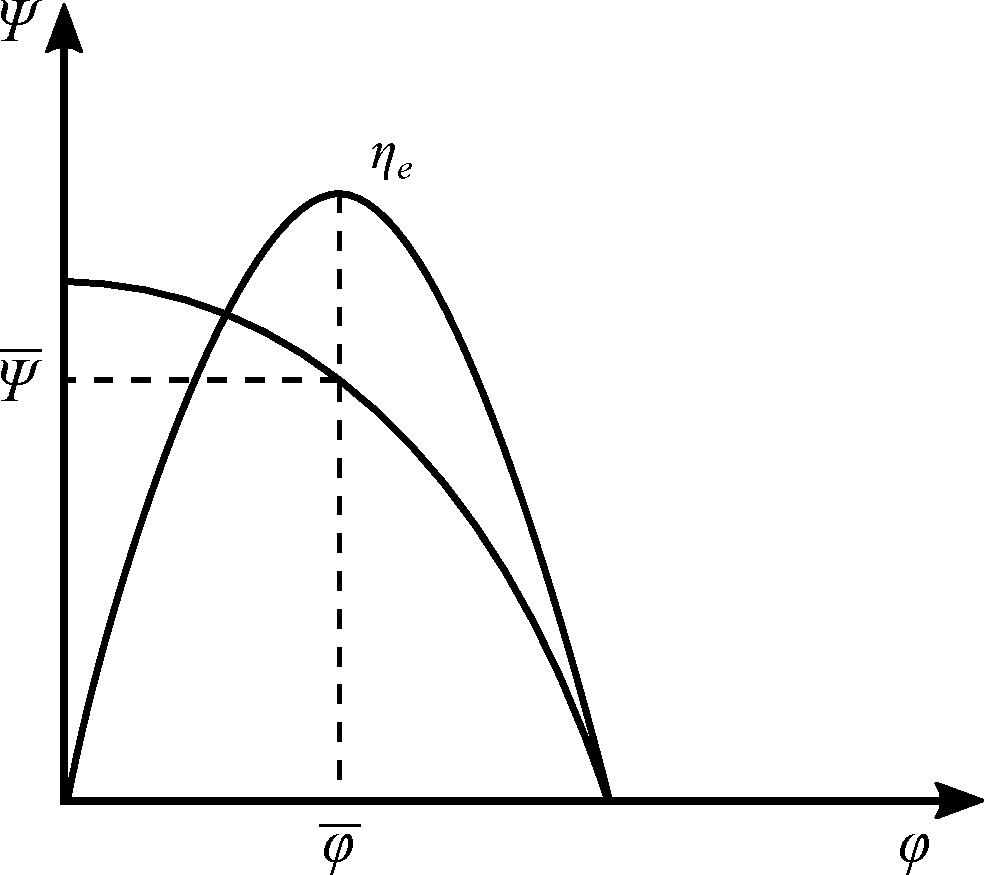
\includegraphics[width=.3\textwidth]{fig/adim.pdf}
\caption{}
\label{fig:adim}
\end{figure}
\begin{equation}
k_P = \frac{w D}{\sqrt{L_i}}
\end{equation}
Si tratta di una cifra che lega la velocità periferica della macchina al lavoro unitario della stessa.

Considerando $\varphi$ e $\psi$ si definisce una cifra di potenza adimensionalizzata come:
\begin{equation}
\Lambda = \frac{P_e}{\rho w^3 D^5} = \varphi \psi
\end{equation}
Introducendo il rendimento, per una macchina motrice vale (si moltiplica perché una parte della portata rilevata all'esterno è passata attraverso i giochi tra cassa e girante senza produrre lavoro utile):
\begin{equation}
\Lambda = \varphi \psi \eta_e
\end{equation}
e per macchina operatrice vale (si divide perché la portata elaborata dalla pompa è leggermente superiore a quella effettivamente fornita all'utilizzatore visto che a causa dei giochi tra cassa e girante una parte del fluido viene ri-aspirata):
\begin{equation}
\Lambda = \frac{\varphi \psi}{\eta_e}
\end{equation}

Con la seguente espressione si può poi eliminare la caratteristica geometrica ottenendo la velocità specifica o numero specifico di macchina; questo rappresenta una condizione di funzionamento portata - lavoro indipendente dalla dimensione della macchina:
\begin{equation}
w_s = k = \varphi^{1/2} \psi^{-3/4} = w \frac{\sqrt{Q}}{L_i^{3/4}}
\end{equation}
La forma della macchina varierà al variare di k. Avere dei coefficienti k piccoli significa avere delle macchine nelle quali il termine di scambio di energia è prevalente rispetto al termine di portata. Questo numero permette, grazie all'esperienza storica (ovvero di tutti i dati che il progettista o la sua azienda possiedono in merito alle prestazioni di altre macchine), di classificare la forma geometrica di una macchina in base alle condizioni portata - lavoro.
\begin{figure}[h!]
\centering
  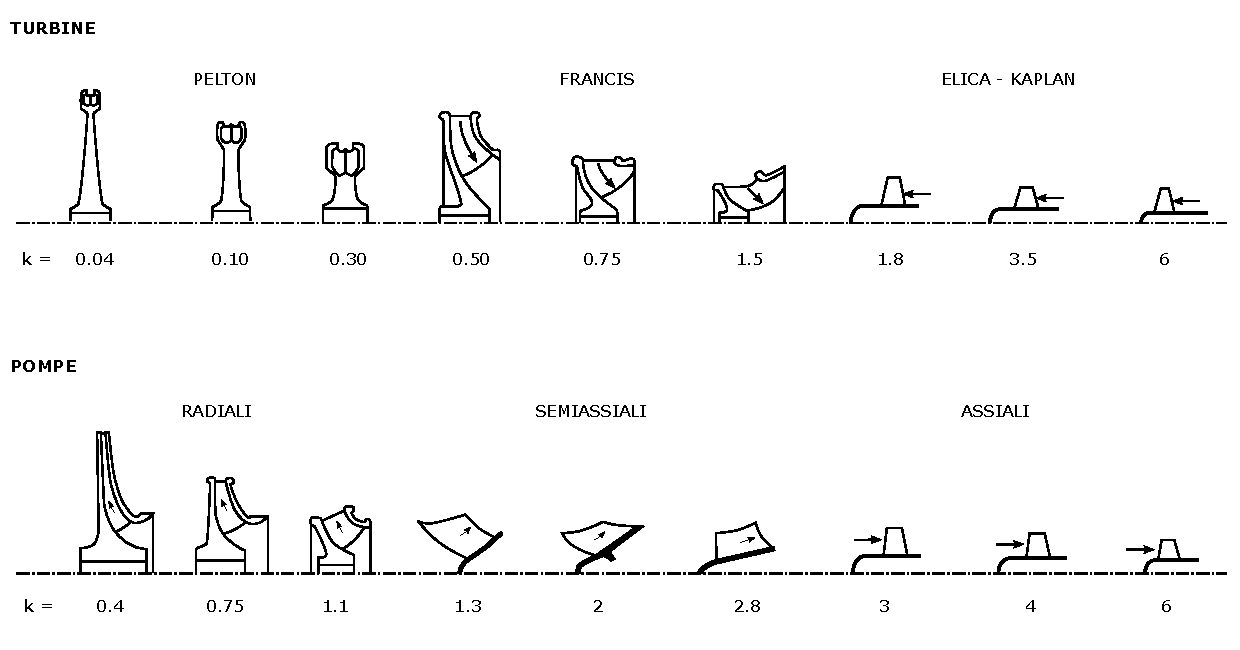
\includegraphics[width=\textwidth]{fig/numcar.pdf}
\caption{Variazione della forma delle giranti delle turbine idrauliche al variare del numero caratteristico di macchina.}
\label{fig:numcar}
\end{figure}

Sfruttando l'esperienza si analizzano le migliori macchine esistenti e si vede quanto valgono per quelle macchine le cifre adimensionali $\pi_i$, $\pi_j$ e si diagrammano in funzione di k. Facendo un esempio concreto si considera una tipica macchina radiale (una pompa centrifuga) e se ne analizza la sezione meridiana semplificata al massimo (figura \ref{fig:pala}).
\begin{figure}
\centering
\begin{minipage}{.5\textwidth}
  \centering
  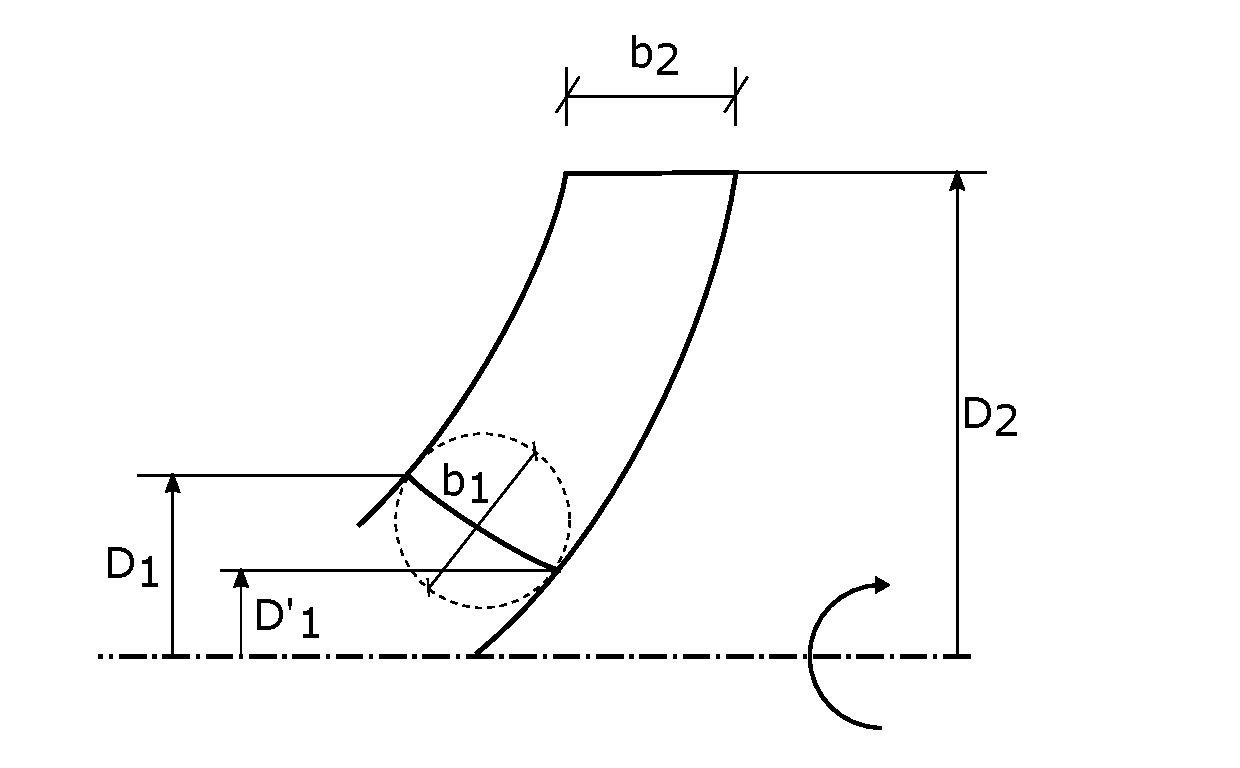
\includegraphics[width=.9\linewidth]{fig/pala.pdf}
  \captionof{figure}{}
  \label{fig:pala}
\end{minipage}%
\begin{minipage}{.5\textwidth}
  \centering
  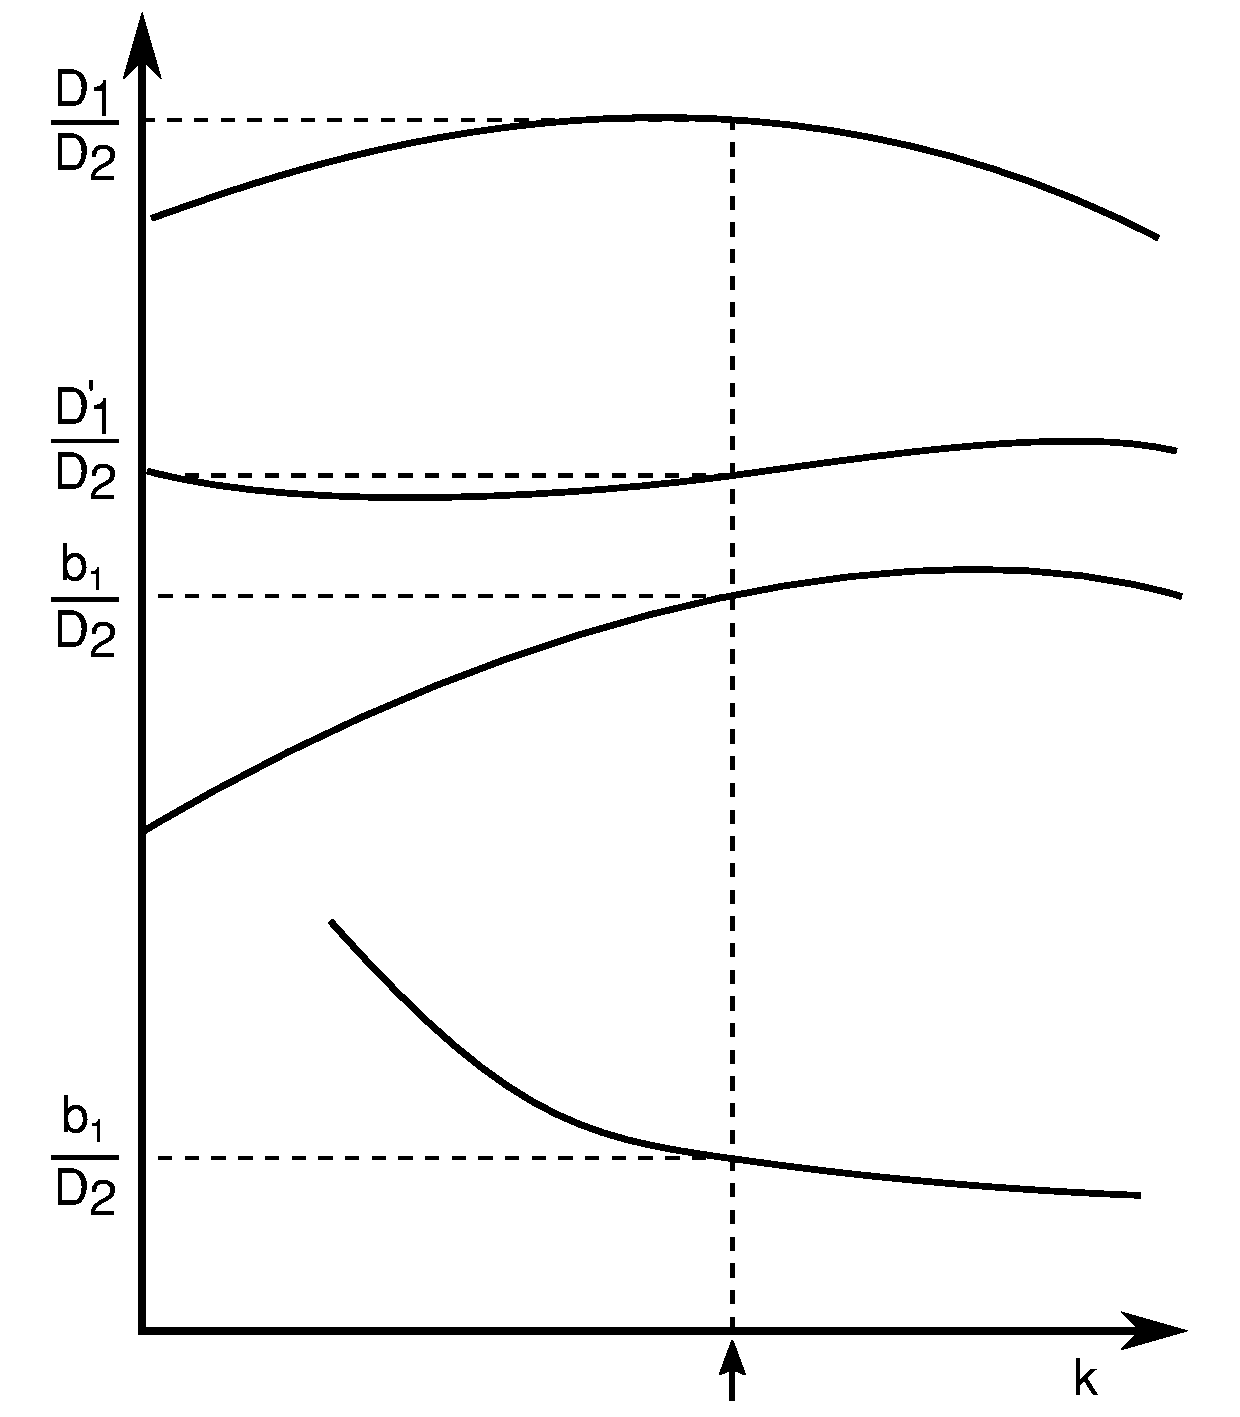
\includegraphics[width=.6\linewidth]{fig/primo_1.pdf}
  \captionof{figure}{}
  \label{fig:primo_1}
\end{minipage}
\end{figure}
\\Si definiscono le seguenti dimensioni caratteristiche più significative (si tratta di un esempio didattico, in realtà si può definire un database molto più ampio e raffinato):
\begin{itemize}
\item[-]$D_2$: diametro massimo della girante;\\
\item[-]$D_1$: diametro massimo della sezione di ingresso;\\
\item[-]$D_1^{'}$: diametro minimo della sezione d'ingresso;\\
\item[-]$b_2$: altezza della pala in uscita;\\
\item[-]$b_1$: altezza della pala in ingresso.
\end{itemize}
Per definire $b_1$ bisogna considerare il diametro medio e con riferimento al punto di intersezione tra questo ed il profilo della pala in ingresso, si traccia la circonferenza inscrivibile nella sezione d’ingresso. Come grandezza caratteristica della sezione d’ingresso si prende proprio il diametro di questa circonferenza. Per queste grandezze si definiscono i seguenti rapporti adimensionali:
\begin{align*}
\frac{D_1}{D_2} \;\;\; \frac{D_1^{'}}{D_2} \;\;\; \frac{b_1}{D_2} \;\;\; \frac{b_2}{D_2} 
\end{align*}
Essi sono funzioni di $k$ e quindi si riescono a definire delle curve che riportano in ascissa il valore del numero caratteristico $k$ e in ordinata i valori dei quattro rapporti (figura \ref{fig:primo_1}).\\
Ricapitolando: note portata e prevalenza e fissata la velocità di rotazione, è noto il valore di $k$. Utilizzando questi diagrammi si trovano i valori dei quattro parametri e quindi si definisce per sommi capi la sezione meridiana della macchina in analisi.

Esiste una dimensione ottimale ossia una dimensione alla quale corrisponde il massimo rendimento; va però definita un’ulteriore grandezza detta diametro specifico:
\begin{equation}
D_s= \varphi^{-1/2} \psi^{1/4} = D \cdot \frac{L_i^{1/4}}{\sqrt{Q}}
\end{equation}
È stato verificato che esiste, con riferimento alle dimensioni che danno massimo rendimento, un legame tra $D_s$ e $w_s$.
Questo è descritto empiricamente sul diagramma di Cordier rappresentato in figura \ref{fig:cord_diag}. Questo diagramma rappresenta l’interpolazione di una serie di dati sperimentali (da vedere come correlazione statistica).\\
In figura \ref{fig:primo_3} è invece riportato il diagramma di Balje; grazie alle curve presenti è possibile osservare l’entità delle variazioni che si ottengono andando a discostarsi, entro certi limiti, dalla curva di Cordier che rappresenta la condizione di massimo rendimento.
\begin{figure}
\centering
\begin{minipage}{.5\textwidth}
  \centering
  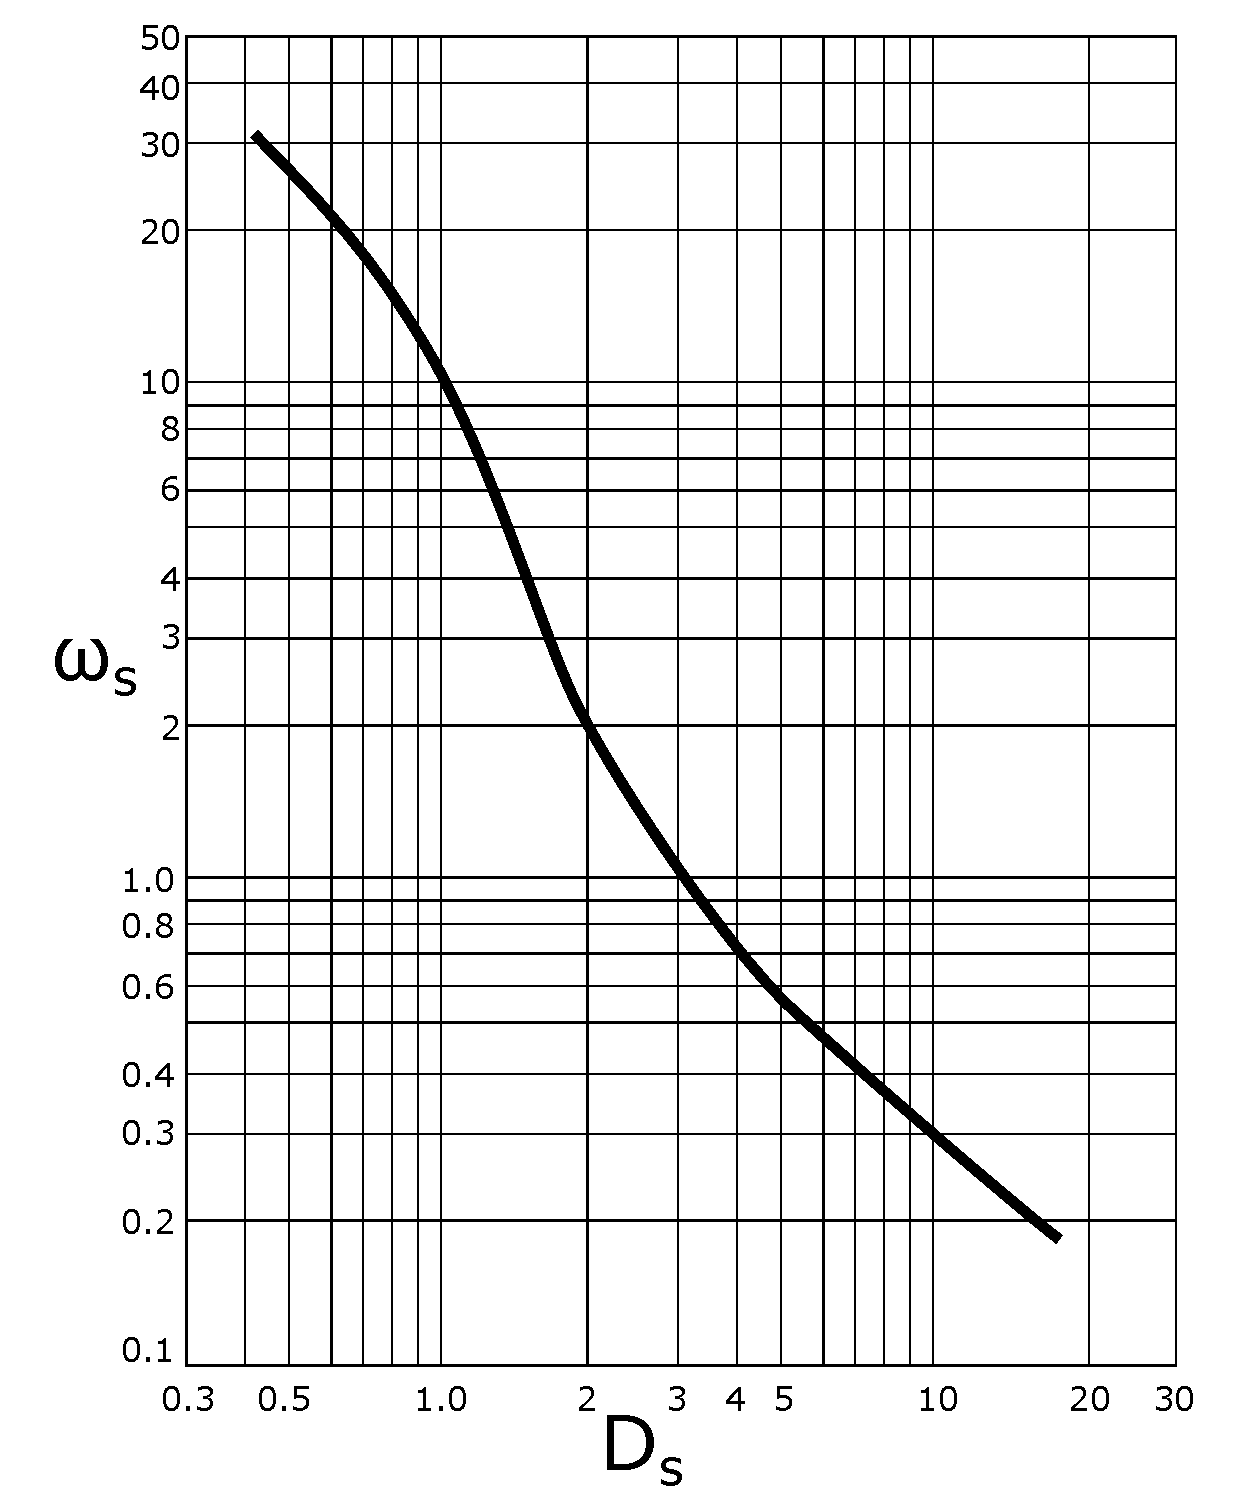
\includegraphics[width=.95\linewidth]{fig/cord_diag.pdf}
  \captionof{figure}{Diagramma di Cordier}
  \label{fig:cord_diag}
\end{minipage}%
\begin{minipage}{.5\textwidth}
  \centering
  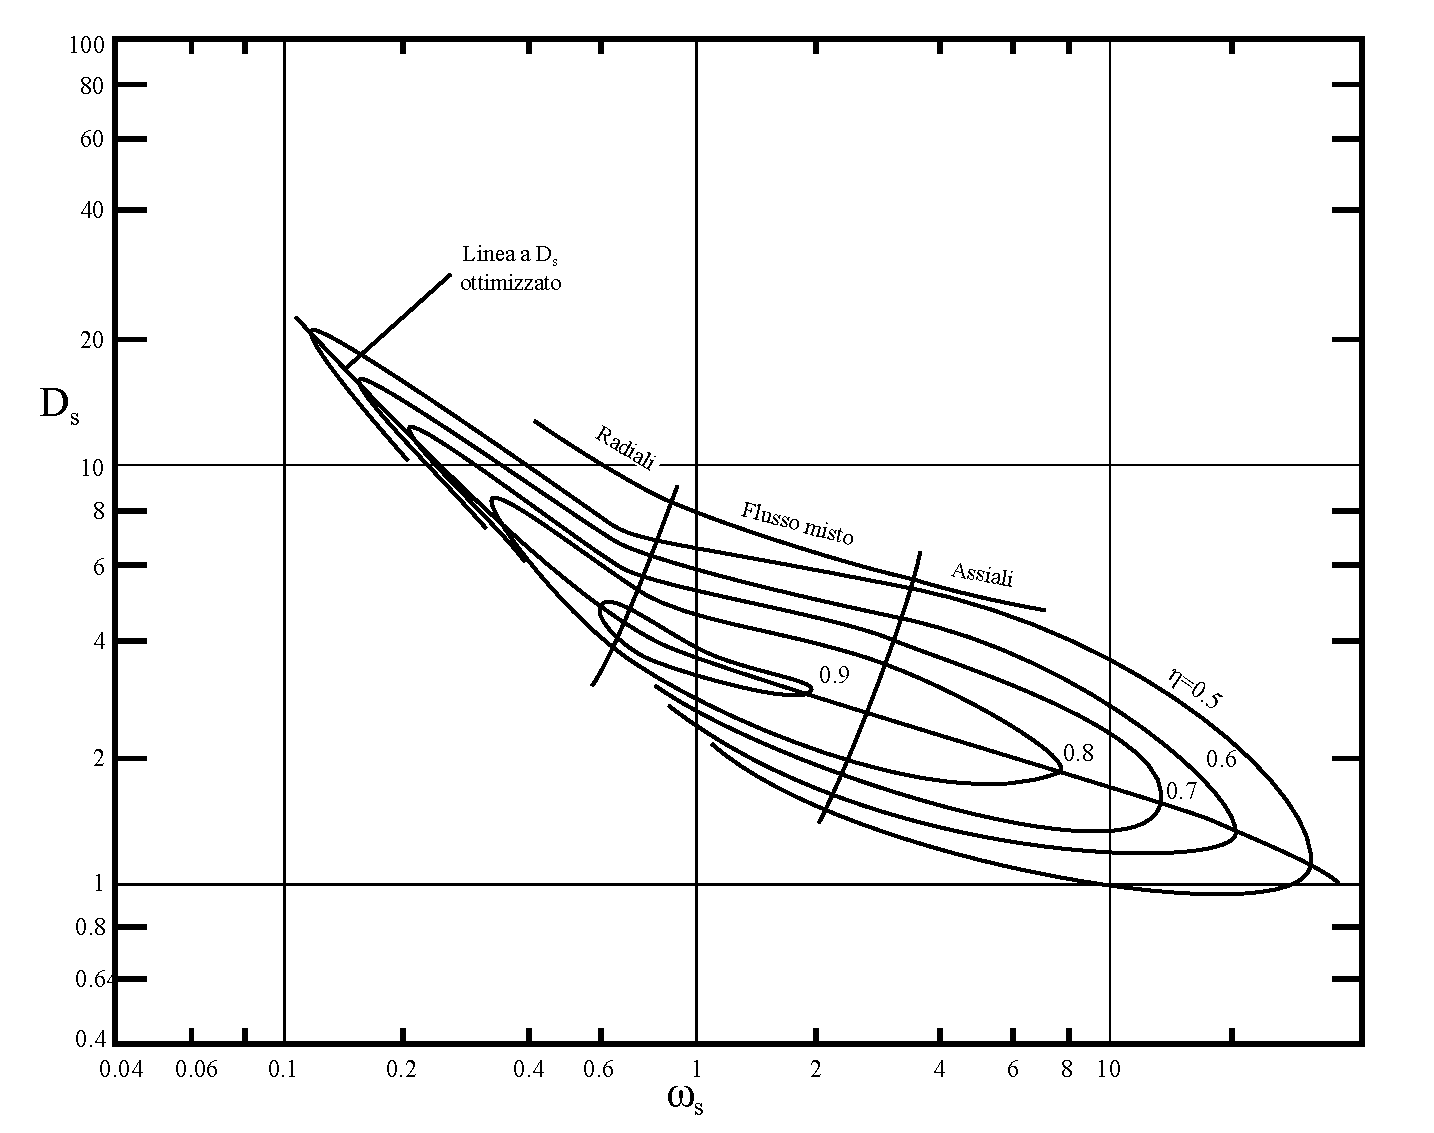
\includegraphics[width=\linewidth]{fig/primo_3.pdf}
  \captionof{figure}{Diagramma di Balje}
  \label{fig:primo_3}
\end{minipage}
\end{figure}
\section{Influenza di Re}
Tutte queste considerazioni sono state fatte trascurando l'influenza di Re. Il diagramma di Moody (\ref{fig:moody}) è costruito considerando valori diversi di $\epsilon/D$. Per le macchine questo rapporto è essenzialmente costante e si può notare nel diagramma come al diminuire di Re le curve si spostino più in alto; questo effetto si riflette in un abbassamento di rendimento e quindi della prevalenza.\\
Questo è un fenomeno prevedibile in termini statistici e, storicamente, grazie all'accumulazione di dati sperimentali, sono stati definiti due fattori di correzione:
\begin{itemize}
	\item fattore di correzione per il rendimento: $f_\eta$
	\item fatto di correzione per la cifra di pressione: $f_\psi$
\end{itemize} 
Questi sono stati diagrammati rispetto a $Re$. Man mano che $Re$ diminuisce il loro effetto diventa sempre più importante (figura \ref{fig:secondo_2}). 
\begin{figure}
\centering
\begin{minipage}{.4\textwidth}
  \centering
  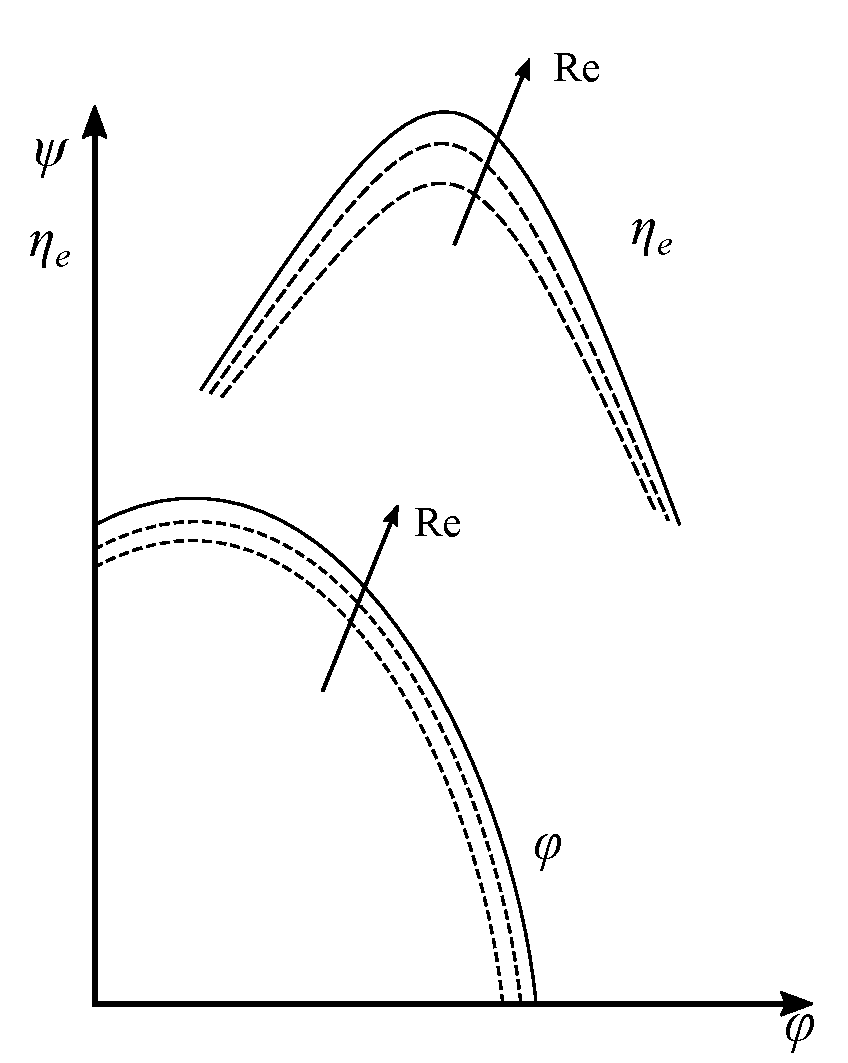
\includegraphics[width=.95\linewidth]{fig/secondo_1.pdf}
  \captionof{figure}{}
  \label{fig:secondo_1}
\end{minipage}%
\begin{minipage}{.6\textwidth}
  \centering
  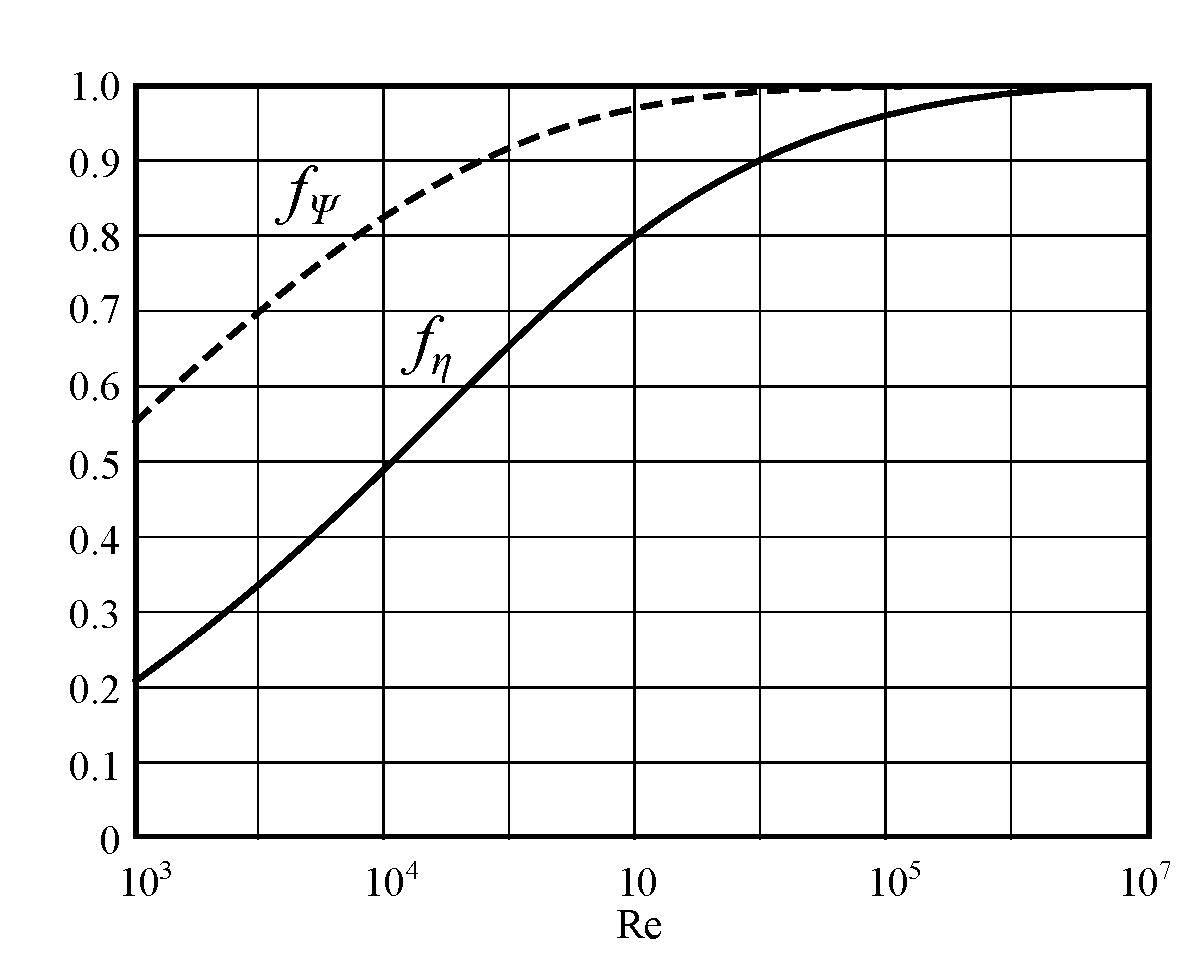
\includegraphics[width=.95\linewidth]{fig/secondo_2.pdf}
  \captionof{figure}{}
  \label{fig:secondo_2}
\end{minipage}
\end{figure}
\\Partendo dalla definizione di $w_s$, si scrivono $\varphi$ e $\psi$ nei diversi punti di funzionamento della macchina in funzione di $w_s$:
\begin{align*}
w_s= \varphi^{1/2}\psi^{-3/4} \;\;\;\; \Rightarrow \;\;\;\;
\begin{cases}
\psi = \psi(w_s)\\
\eta = \eta(w_s)
\end{cases} \;\;\;\;\;\;\;\;
\begin{cases}
f_{\psi} = f(Re)\\
f_{\eta} = f(Re)
\end{cases}
\end{align*}
Grazie ai coefficienti correttivi si trovano le cifre adimensionali corrette:
\begin{align*}
\begin{cases}
\psi_{corretto} = f_{\psi} \cdot \psi(w_s)\\
\eta_{corretto} = f_{\eta} \cdot \eta(w_s)
\end{cases}
\end{align*}
A questo punto è possibile procedere a ritroso. Trovato il valore corretto si ricalcola $\omega_s$:
\begin{align*}
\omega_s = \varphi^{1/2} \psi^{-3/4} =  \varphi^{1/2} \psi_{corretto}^{-3/4} = cost
\end{align*}
e partendo dal suo valore è possibile costruire le curve di prestazione corrette.
\section{Effetto scala}
A parità di bontà di progettazione, geometria, ecc, una macchina grande ha un rendimento maggiore rispetto ad una macchina piccola. Questo si spiega facendo due osservazioni: 
\begin{enumerate}
	\item a parità di tecnologia produttiva è possibile ritenere costante il valore della rugosità superficiale delle palettature della girante. In una macchina grande la rugosità relativa ($\epsilon/D$) sarà quindi più bassa, quindi le perdite di carico saranno superiori nella macchina piccola;
	\item bisogna considerare i giochi presenti tra parte fissa e parte mobile, che non possono scendere al di sotto di un certo limite. Nelle macchine grandi questi diventeranno trascurabili. 
\end{enumerate}
\begin{figure}
\centering
  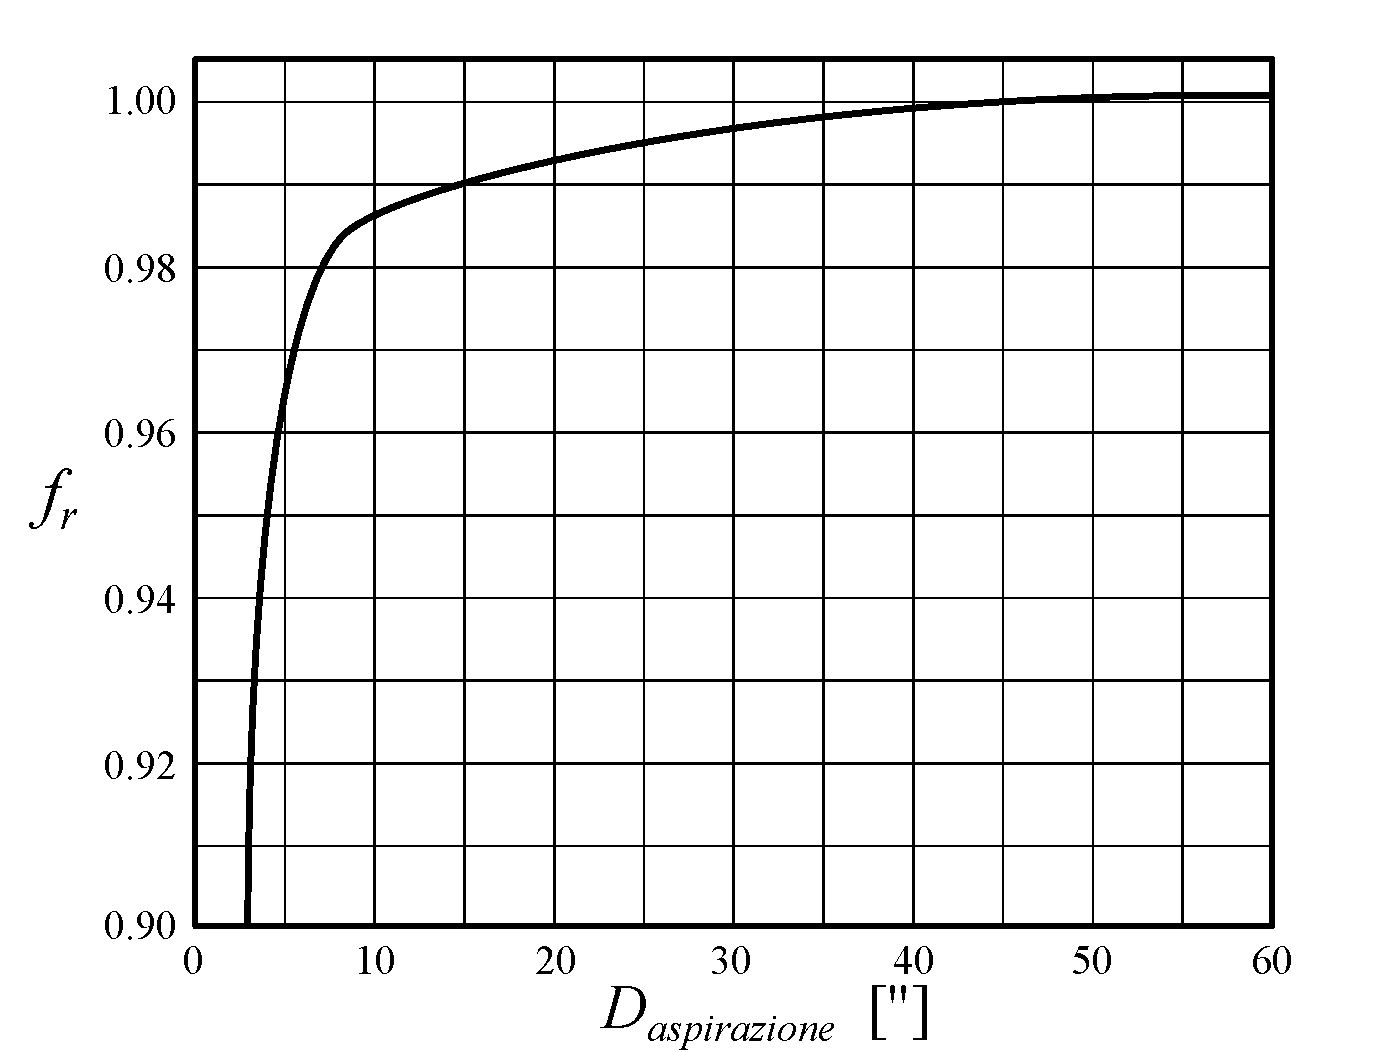
\includegraphics[width=.5\textwidth]{fig/dDchart.pdf}
\caption{}
\label{fig:dDchart}
\end{figure}
L'effetto scala può essere espresso rispetto ai rapporti dimensionali per via empirica sulla base dei dati storici. Facendo riferimento alle pompe si definisce un rapporto dimensionale:
\begin{align*}
\frac{D_1}{D_2} \triangleq  \mbox{Rapporto di scala} \;\;\;\; \text{con } D_1 < D_2
\end{align*}
Per considerare l'influenza del diametro sul rendimento, facendo riferimento al grafico in figura \ref{fig:dDchart}, il rendimento di una macchina si può esprimere come:
\begin{align*}
\eta = \eta_S \cdot f_r(D)
\end{align*}
con $\eta_S$ il rendimento standard e $f_r$ un coefficiente correttivo funzione del diametro.\\
Considerando due pompe con scala diversa, la relazione tra il loro rendimento è:
\begin{equation}
\frac{1-\eta_1}{1-\eta_2} = \left( \frac{D_2}{D_1}\right)^\alpha
\end{equation}
La stessa operazione viene fatta anche per le turbine idrauliche:
\begin{center}
\begin{tabular}{l l l l l l l l}
	$\cfrac{1-\eta_1}{1-\eta_2} = \left[ \cfrac{Re_{u,2}}{Re_{u,1}} \right]^n$ & & & & & & & $n=0.1 \div 0.25$\\
	$\cfrac{1-\eta_1}{1-\eta_2} =0.5 + 0.5 \left[ \cfrac{Re_{u,2}}{Re_{u,1}} \right]^{0.2}$ & & & & & & & formula di Ackeret, usata in Europa\\
	$\cfrac{1-\eta_1}{1-\eta_2} = 0.3 + 0.7 \left[ \cfrac{Re_{u,2}}{Re_{u,1}} \right]^{0.2}$ & & & & & & & usata per turbine Kaplan\\
\end{tabular}
\end{center}
\section{Flusso comprimibile}
Se si considera il flusso comprimibile le relazioni diventano più complesse. Infatti si ha:
\begin{equation}
\psi=f(\varphi,Ma)
\end{equation}
Nel diagramma $\varphi-\psi$ si ottengono diverse curve al variare del numero di Mach (Figura \ref{fig:ComprMach}) e perciò il grafico diventa di difficile lettura e comprensione. Infatti, per diversi valori delle grandezze termodinamiche di temperatura e pressione, risulta possibile ottenere le stesse quantità di lavoro unitario e ciò comporta una mancata definizione univoca dello stesso. Si tratta però di una rappresentazione poco fisica e di un esercizio esclusivamente accademico.
\begin{figure}[h!]
\centering
  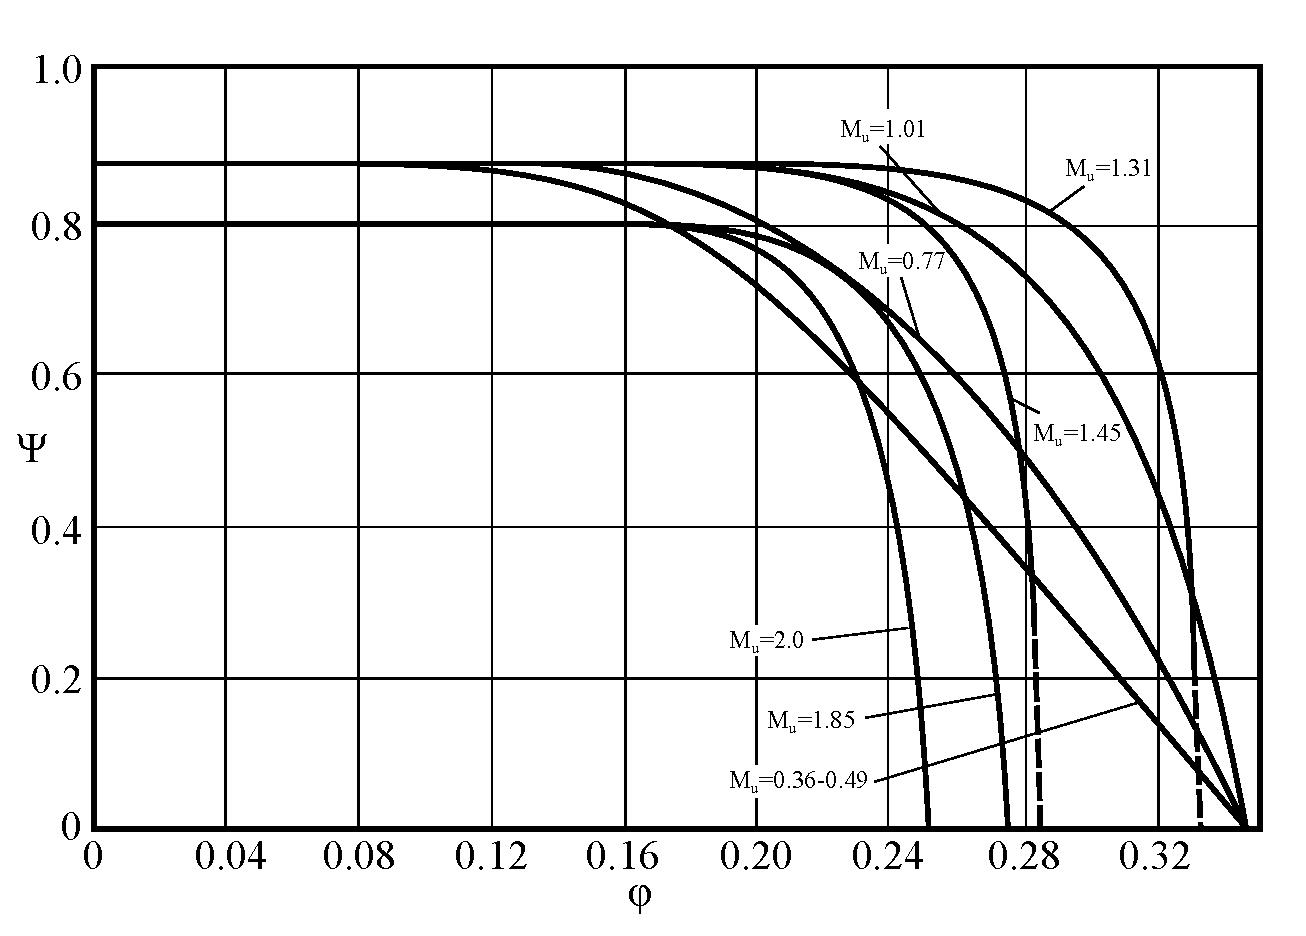
\includegraphics[width=.85\textwidth]{fig/ComprMach.pdf}
\caption{Curve adimensionali di funzionamento di una famiglia di compressori, per un fluido assegnato, a diversi numeri di Mach periferici. Sono definiti $Ma = \frac{w \frac{D}{2}}{a_{01}}$, $Mu = \frac{w \frac{D}{2}}{a}$}
\label{fig:ComprMach}
\end{figure}
\\Per avere una grandezza confrontabile di funzionamento bisogna effettuare tutte le prove in condizioni standard; in questo modo si riesce a rappresentare le condizioni di funzionamento in modo univoco.

Considerando un gas generico miscela di due gas con massa molare $M_i$ \footnote{Nota bene: solo in questo contesto si utilizza $M$ per indicare la massa molare, in tutto il resto del libro viene usato per indicare il numero di Mach.} si può scrivere:
\begin{align*}
\frac{p}{\rho} = \frac{p_1}{\rho} + \frac{p_2}{\rho} = x_1  \frac{p_1}{\rho_1} + x_2  \frac{p_2}{\rho_2} = RT \left( \frac{x_1}{M_1} + \frac{x_2}{M_2} \right) = RT\left(\frac{1}{M_{tot}}\right)
\end{align*}
\begin{align*}
c_p = x_1 c_{p1} + x_2 c_{p2}
\end{align*}
con:\\[1mm]
$M_{1/2/tot}$: numero di moli\\
$x_{1/2}$: frazione molare\\
$R$: costante dei gas perfetti\\[2mm]
Si ricorda poi che definiti calore specifico a pressione costante $c_p$ e calore specifico a volume costante $c_v$ si ha:
\begin{align*}
\gamma = \frac{c_p}{c_v} \;\;\;\;\;\; R = c_p - c_v
\end{align*}
\begin{align*}
\cfrac{\gamma}{\gamma -1} = \cfrac{\cfrac{x_1}{M_1} \cfrac{\gamma_1}{\gamma_1 -1}+\cfrac{x_2}{M_2} \cfrac{\gamma_2}{\gamma_2 -1}}{\cfrac{x_1}{M_1}+\cfrac{x_2}{M_2}}
\end{align*}
Si definisce il significato dei pedici:
\begin{itemize}
	\item $s$: grandezze relative alle condizioni standard;
	\item $c$: valori corretti, cioè riportati alle condizioni standard;
	\item ``  ": valori da correggere rilevati nel corso della prova.
\end{itemize}
Di seguito vengono riportate le grandezze significative corrette rispetto alle condizioni standard:
\begin{itemize}
	\item \textbf{Rapporto di compressione}:
	\begin{align*}
	\frac{p_{02}}{p_{01}} = \frac{p_{02c}}{p_{01s}} \;\;\;\; \Rightarrow \;\;\;\; p_{02c} = p_{02}\frac{p_{01s}}{p_{01}}
	\end{align*}
	\item \textbf{Parametro di portata}:
	\begin{align*}
	\frac{\dot{m}\sqrt{T_{01}}}{p_{01}}=\frac{\dot{m_c}\sqrt{T_{01s}}}{p_{01s}} \;\;\;\; \Rightarrow \;\;\;\; \dot{m_c} = \dot{m} \sqrt{\frac{T_{01}}{T_{01s}}} \bigg(\frac{p_{01s}}{p_{01}} \bigg)
	\end{align*}
	\item \textbf{Parametro di velocità}:
	\begin{align*}
	\frac{n}{\sqrt{T_{01}}}=\frac{n_c}{\sqrt{T_{01s}}} \;\;\;\; \Rightarrow \;\;\;\; n_c = n \sqrt{\frac{T_{01s}}{T_{01}}}
	\end{align*}
	\item \textbf{Pressione ridotta}:
	\begin{align*}
	\delta = \frac{p_{01}}{p_{01s}}
	\end{align*}
	\item \textbf{Temperatura ridotta}:
	\begin{align*}
	\theta = \frac{T_{01}}{T_{01s}}
	\end{align*}
\end{itemize}
Considerando le espressioni precedenti si possono esprimere più sinteticamente le grandezze corrette:
\begin{align*}
p_{02c} = \frac{p_{02}}{\delta} \;\;\;\;\;\;\;\; \dot{m_c}= \dot{m} \frac{\sqrt{\theta}}{\delta} \;\;\;\;\;\;\;\; n_c = \frac{n}{\sqrt{\theta}}
\end{align*}
ottenendo così la pressione corretta in aspirazione, la portata di massa corretta e il numero di giri corretto.
\begin{figure}
	\centering
	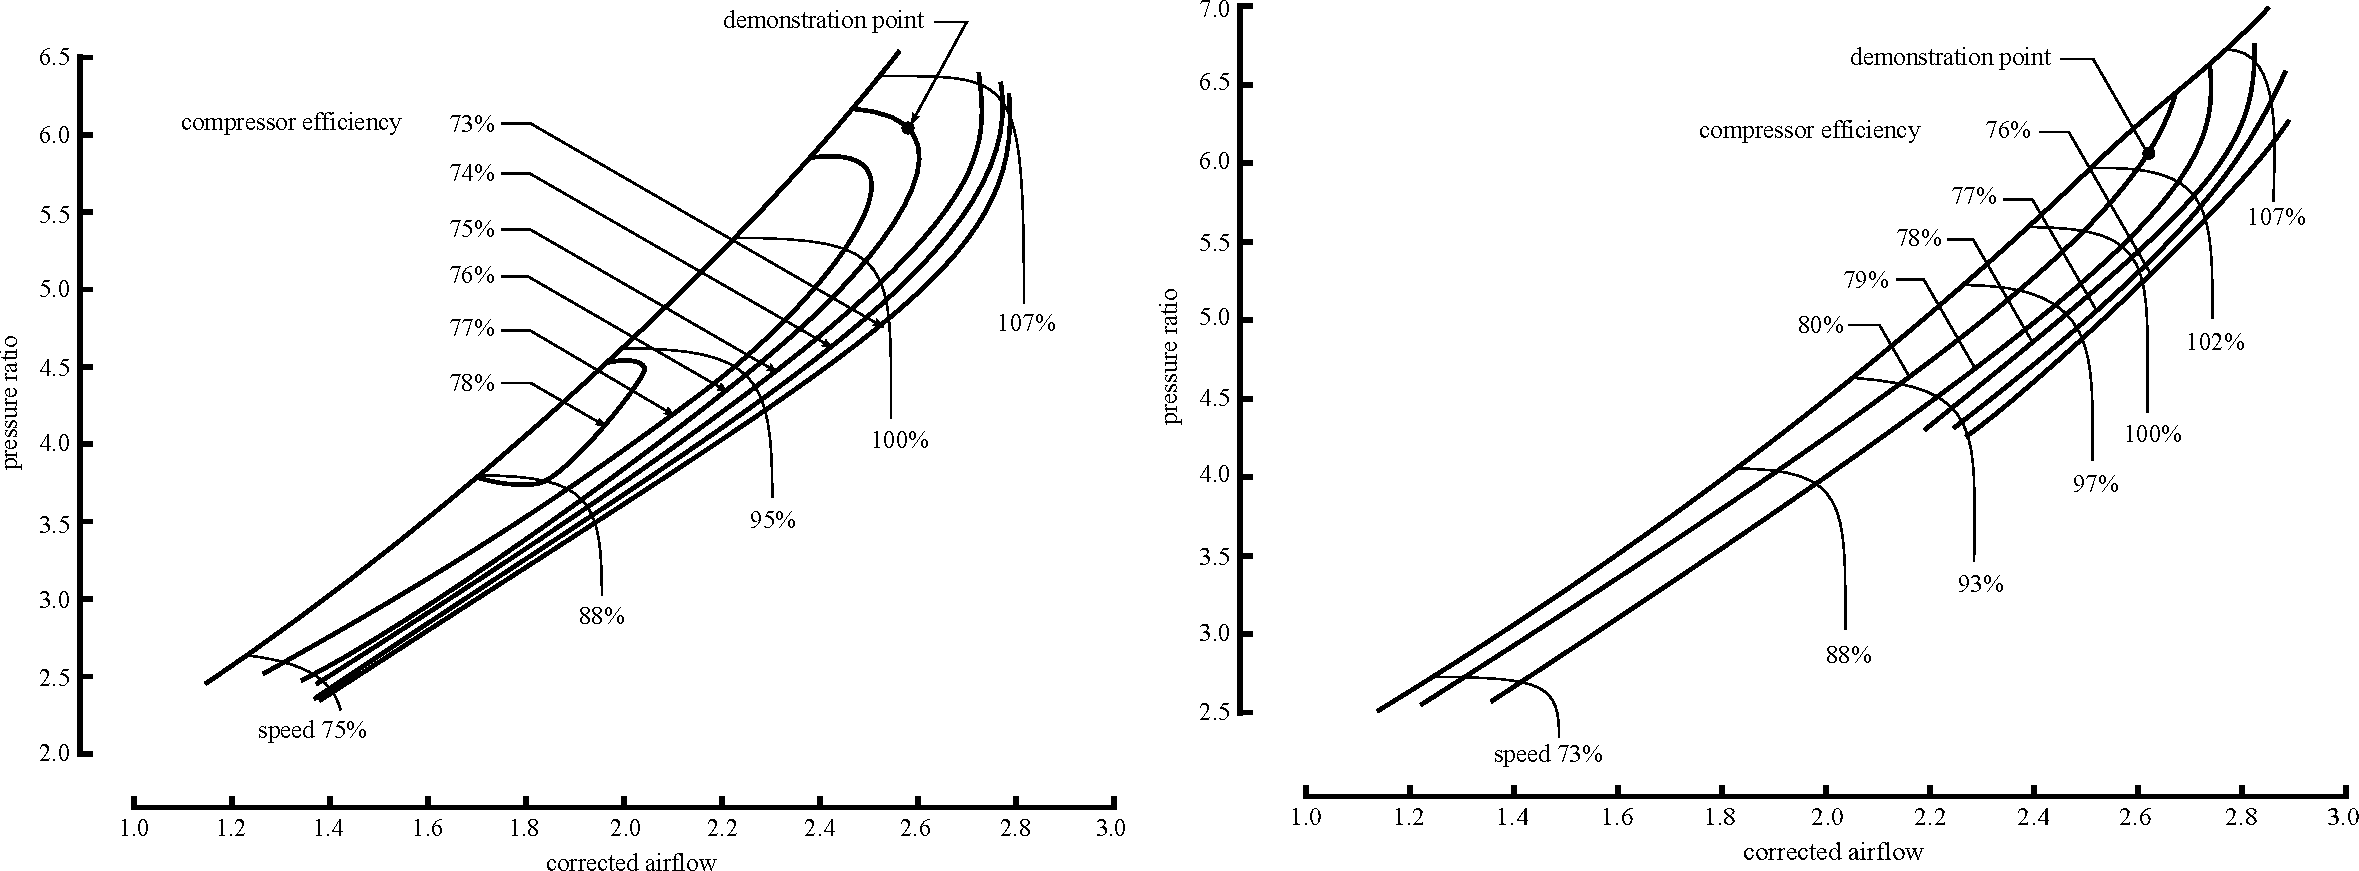
\includegraphics[width=\textwidth]{fig/CompMaps.pdf}
	\caption{}
	\label{fig:compMaps}
\end{figure}
\\In questo modo si trovano le mappe di funzionamento delle macchine (figura \ref{fig:compMaps}) diagrammando la portata d'aria corretta con il rapporto di compressione; sono tracciate diverse curve di isorendimento al variare del numero di giri.

Considerando un compressore se ne vuole rappresentare in modo univoco il comportamento usando i termini $\varphi$ e $\psi$ ma mantenendo la significatività fisica. Si espande l'espressione di $\varphi$ tenendo conto delle seguenti espressioni di $M_{01}$, $p$ e $a$:
\begin{align*}
a = \sqrt{k R T} \;\;\;\;\;\;\;\; M_{01}=\frac{w D}{a_{01}}= \frac{w D}{\sqrt{k R T_{01}}} \;\;\;\;\;\;\;\; p = \rho_i RT 
\end{align*}
\begin{equation}
\varphi = \frac{\dot{m}}{\rho_{01} w D^3} = \frac{\dot{m}}{\rho_{01} M_{01} a_{01} D^2} = \frac{\dot{m} R T_{01}}{p_{01} M_{01} \sqrt{k R T_{01}} D^2} = \frac{\dot{m} \sqrt{R T_{01}}}{p_{01} M_{01} \sqrt{k} D^2}
\end{equation}
La cifra $\psi$ è esprimibile in funzione di $M_{01}$, del rapporto di compressione e delle caratteristiche del fluido ($k$):
\begin{equation}
\psi = \cfrac{L_i}{w^2 D^2} = \cfrac{\Delta h_{0s}}{w^ 2 D^2} = \cfrac{\cfrac{k}{k-1} R T_{01}\left[ \bigg( \cfrac{p_{02}}{p_{01}} \bigg)^{\frac{k-1}{k}}-1\right]}{M_{01}^2 k R T_{01}} = \cfrac{\cfrac{1}{k-1} \left[ \bigg( \cfrac{p_{02}}{p_{01}} \bigg)^{\frac{k-1}{k}}-1\right]}{M_{01}^2 }
\end{equation}
Si possono fare alcune ipotesi semplificative:
\begin{itemize}
	\item Utilizzando lo stesso fluido si possono trascurare $R$ e $k$.
	\item Utilizzando la stessa macchina si trascura $D$.
	\item Riferendosi alle condizioni standard $M_{01}=cost$.
\end{itemize}
Si perviene quindi le seguenti relazioni semplificate:
\begin{align*}
M_{01}=\frac{w D}{\sqrt{k R T_{01}}} \;\;\;\;\;\;\;\; \Rightarrow \;\;\;\;\;\;\;\; M_{01}=\frac{w}{\sqrt{T_{01}}}=cost
\end{align*}
\begin{align*}
\varphi=\frac{\dot{m} \sqrt{RT_{01}}}{p_{01} M_{01} \sqrt{k}D^2} \;\;\;\;\;\;\;\; \Rightarrow \;\;\;\;\;\;\;\; \varphi=\frac{\dot{m} \sqrt{T_{01}}}{p_{01}}
\end{align*}
\begin{align*}
\psi= \cfrac{\cfrac{1}{k-1} \left[ \bigg( \cfrac{p_{02}}{p_{01}} \bigg)^{\frac{k-1}{k}}-1\right]}{M_{01}^2 } \;\;\;\;\;\;\;\; \Rightarrow \;\;\;\;\;\;\;\; \psi=\frac{p_{02}}{p_{01}}
\end{align*}
Si tratta di grandezze misurabili in un banco prova.\\
La mappa di funzionamento del compressore assume quindi una forma più leggibile: sull'asse delle ascisse c'è la portata in massa corretta con la temperatura in ingresso (cifra di flusso) e su quello delle ordinate il rapporto di compressione (cifra di pressione). Assieme a queste curve si costruiscono le linee di isorendimento e quindi la curva ideale operativa del compressore data dall'inviluppo delle curve di isorendimento.
\begin{figure}
\centering
  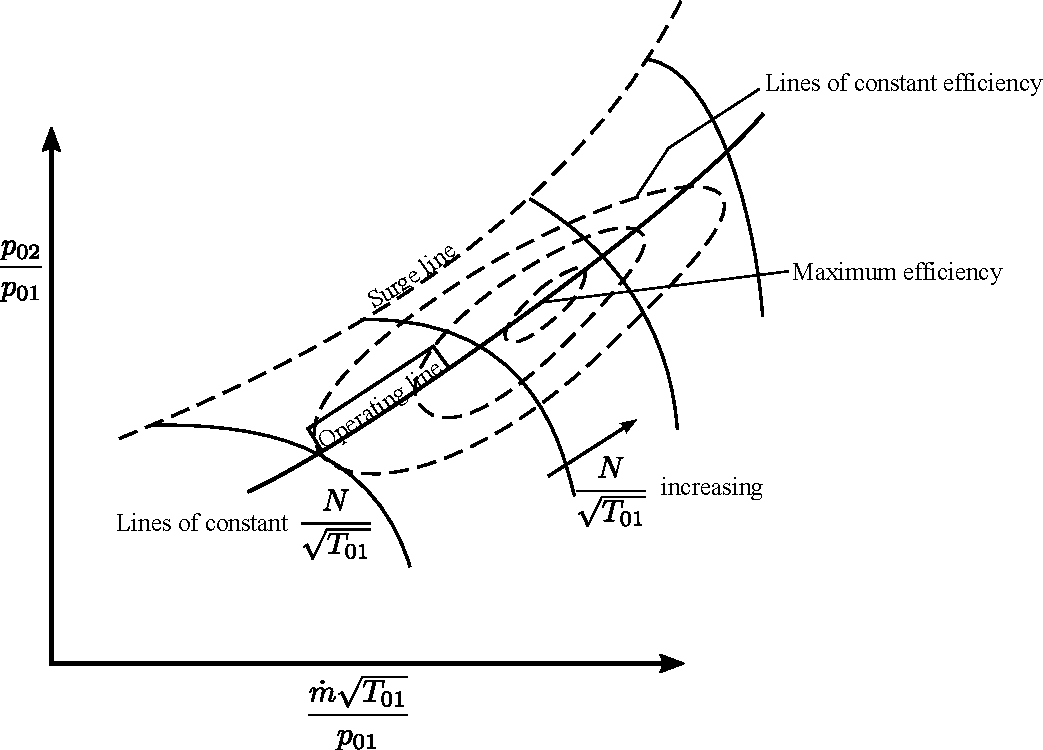
\includegraphics[width=.8\textwidth]{fig/secondo_8.pdf}
\caption{}
\label{fig:secondo_8}
\end{figure}
\\Guardando al diagramma in figura \ref{fig:secondo_8} si nota il fenomeno dell'ingolfamento del compressore; esso si verifica nella zona in cui le linee a velocità costante tendono a diventare verticali. Raggiunta questa condizione non è più possibile variare la portata variando il rapporto delle pressioni; questo si verifica perché in qualche punto si raggiungono le condizioni di flusso sonico e quindi, ricordando lo studio dell'ugello convergente - divergente, si verifica un
blocco sonico delle portata.\\
L'obiettivo è quello di lavorare il più possibile vicino alla ``operating line" che è la zona di massimo rendimento; il problema è che ci si trova pericolosamente vicino alla ``surge line". Oltre la surge line si innesca il fenomeno del pompaggio che può danneggiare la macchina e l'impianto irrimediabilmente.
\section{Richiamo di termodinamica}
Lo scambio termico è trascurabile per i bassi tempi di residenza del fluido nel condotto, per questo motivo si considera il rotore adiabatico. In un rotore adiabatico, per il primo principio della termodinamica essendo il flusso di calore nullo, il lavoro è dato dal salto entalpico tra gli stati $1$ e $2$:
\begin{equation}
L_{12}^{'} = h_{t1}-h_{t2}
\end{equation}
\begin{equation}\label{eq:ent_tot}
h_t=h+\frac{c^2}{2}+gz
\end{equation}
con: \\[1mm]
$h_t$: entalpia totale\\
$h$: entalpia statica\\
$c^2/2$: quota cinetica\\
$gz$: quota gravitazionale\\[2mm]
Per una macchina motrice\footnote{Nel caso delle macchine operatrici si invertono i pedici $1$ e $2$ così da avere lavori per convenzione sempre positivi.} si può scrivere:
\begin{equation}\label{eq:L12}
L_{12}^{'} = \begin{cases} u_1 c_{u1}-u_2 c_{u2}\\
\cfrac{c_1^2-c_2^2}{2}+\cfrac{u_1^2-u_2^2}{2}-\cfrac{w_1^2-w_2^2}{2} \end{cases}
\end{equation}
Il lavoro è costituito da una parte cinetica e da una parte statica, come evidenziato dalle espressioni di $L_{12}^{'}$ nelle formule \ref{eq:ent_tot} e \ref{eq:L12}; in particolare, nell'espressione \ref{eq:L12}, la quota parte cinetica dipende dalla componente assoluta della velocità ($c$), mentre quella statica dipende dalle componenti assiale ($u$) e relativa ($w$).\\
Visto che in una macchina puramente assiale si conserva l'omonima componente $u$ della velocità, allora il contributo $u_1^2 - u_2^2$ nell'espressione del lavoro è nullo: per questo una macchina radiale, a parità di numero di stadi e condizioni, elabora più lavoro di una macchina assiale visto che $u_1^2 - u_2^2$ è maggiore di zero.\\
Ponendosi come osservatori relativi rispetto al rotore ed uguagliando le due espressioni per il lavoro si può scrivere:
\begin{equation}
u_1 c_{u1} - u_2 c_{u2} = h_1 + \frac{c_1^2}{2}+gz_1-h_2-\frac{c_2^2}{2}-gz_2
\end{equation}
Si definisce quindi la rotalpia\footnote{Grandezza che rappresenta la conservazione di energia per la girante.} come:
\begin{equation}
I=h+\frac{c^2}{2}+gz-u c_u = cost
\end{equation}
Essa ha valore costante proprio a seguito dell'adiabaticità del rotore.\\
Quindi in un rotore adiabatico $I=cost$ e in uno statore adiabatico $h_t=cost$ visto che non c'è scambio di calore e di lavoro.\\
Tutte le grandezze fin'ora viste possono essere disegnate in un piano $T-s$ o $h-s$.
\section{Rendimenti per i compressori}
Il rendimento è definito qualitativamente come il rapporto tra l'effetto utile ed il lavoro svolto dalla macchina. Sul lavoro svolto non ci sono ambiguità mentre in merito all'effetto utile si possono avere diverse formulazioni.\\
L'effetto utile può essere considerato come il salto entalpico associato al rapporto di compressione tra le pressioni statiche o totali ingresso/uscita, oppure come combinazione tra grandezze statiche e totali tra ingresso e uscita. Le diverse definizioni di rendimento sono sostanzialmente da imputare alle quote cinetiche ingresso/uscita che possono essere contate o meno come effetto utile.
\begin{figure}
\centering
  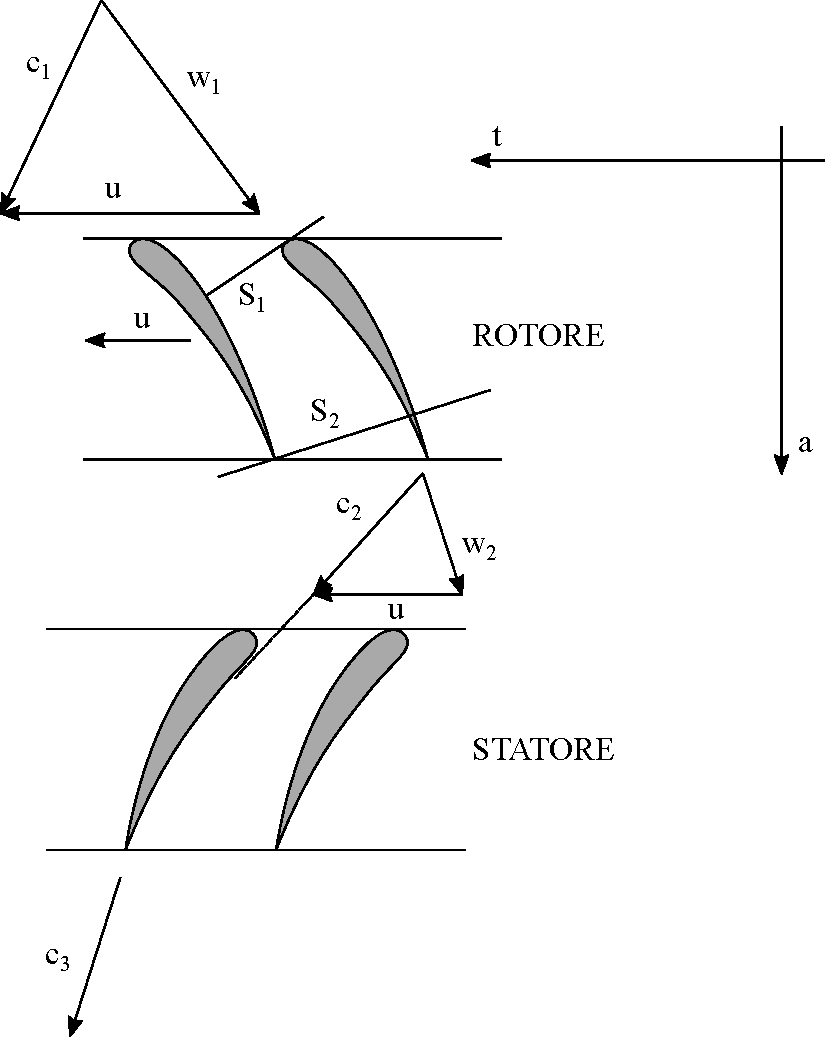
\includegraphics[width=.5\textwidth]{fig/schieraTComp.pdf}
\caption{}
\label{fig:schieraTComp}
\end{figure}

Con riferimento ad una trasformazione di compressione, trascurando i contributi cinetici all'ingresso e all'uscita, si possono definire il rendimento adiabatico ed il rendimento politropico. Tale approccio è spesso utilizzato quando non si vuole entrare nel dettaglio della macchina come invece è necessario fare quando si vogliono studiare le prestazioni dei singoli stadi.\\
Nel caso di rendimento adiabatico (o isoentropico), definendo con $l_{is}$ il lavoro lungo la trasformazione isoentropica e con $l_r$ quello lungo l'adiabatica reale (politropica), e facendo riferimento alla figura \ref{fig:Rend1}, la definizione diventa:
\begin{align*}
\eta_{ad} = \frac{h_{2'} - h_1}{h_2 - h_1} = \frac{c_p \left( T_{2'} - T_1 \right)}{c_p \left( T_2 - T_1 \right)} =
 \frac{\Bigg( \beta^{\cfrac{\gamma -1}{\gamma}} -1 \Bigg)}{\Bigg( \beta^{\cfrac{n -1}{n}} -1 \Bigg)} = \frac{l_{is}}{l_r}
\end{align*}
con:\\[1mm]
$c_p = cost$ con la temperatura e pressione\\
$\beta$: rapporto di compressione\\
$\gamma=c_p/c_v$: indice della trasformazione isoentropica\\
$n=(c_p-c)/(c_v-c)$: indice della trasformazione politropica (corrispondente alla trasformazione reale)\\[2mm]
La scelta di questa definizione, oltre al facile utilizzo, è quella di fornire un'indicazione diretta dello scostamento della trasformazione da quella migliore possibile, l'isoentropica, senza dedicare particolare attenzione alle energie cinetiche presenti all'interno del sistema macchina.
\begin{figure}[h!]
\centering
\begin{minipage}{.45\textwidth}
  \centering
  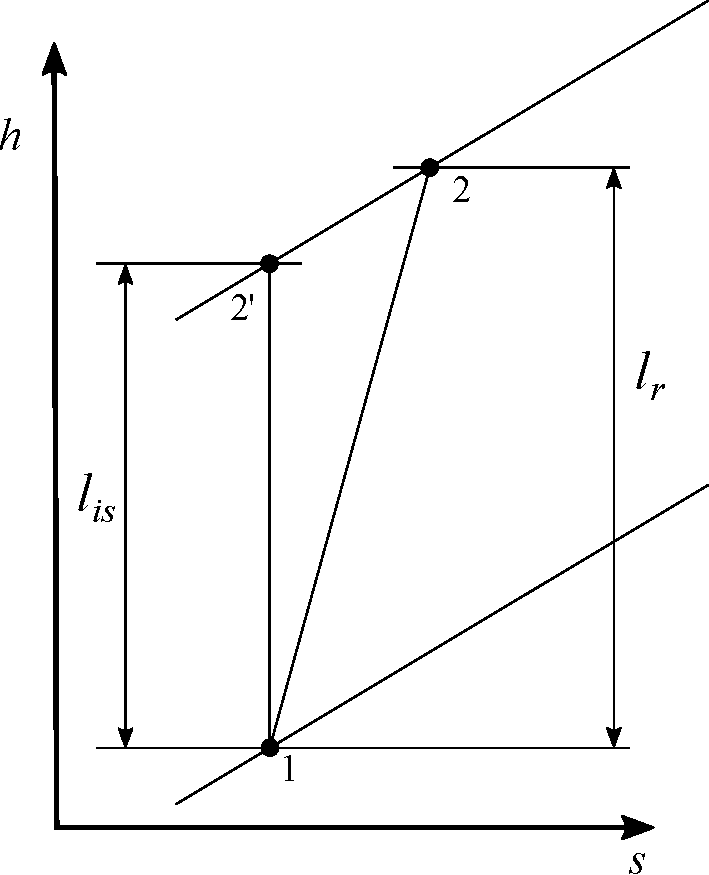
\includegraphics[width=.9\linewidth]{fig/Rend1.pdf}
  \captionof{figure}{}
  \label{fig:Rend1}
\end{minipage}%
\begin{minipage}{.55\textwidth}
  \centering
  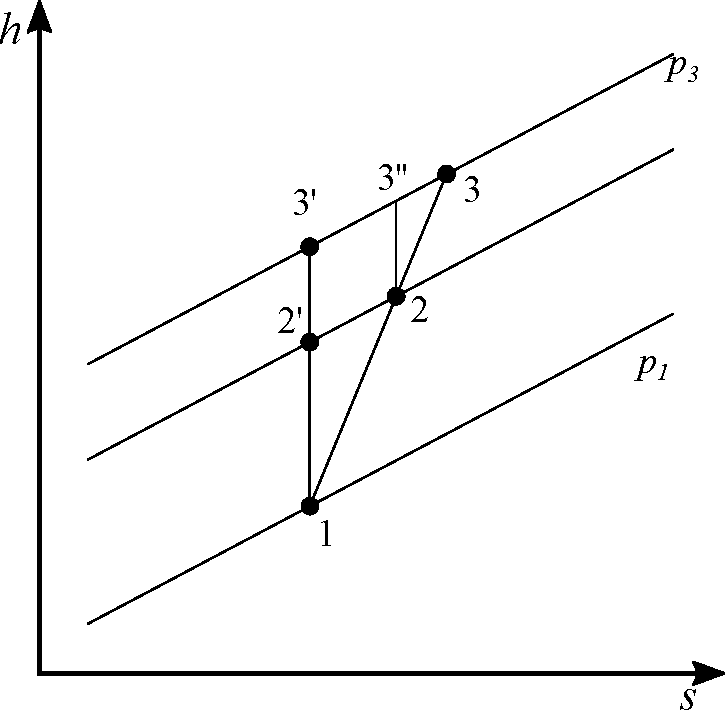
\includegraphics[width=.9\linewidth]{fig/Rend2.pdf}
  \captionof{figure}{}
  \label{fig:Rend2}
\end{minipage}
\end{figure}

Si può considerare poi il rendimento politropico definito dalla trasformazione politropica reversibile tra i punti $1$ e $2$, come riferimento per la trasformazione reale, figura \ref{fig:Rend2}. Questo viene incontro alla necessità, nel caso di macchine multistadio (o a singolo stadio ma con elevato rapporto di compressione), di non imputare ad una porzione di trasformazione la storia dei volumi specifici precedenti ed in particolar modo le irreversibilità precedenti.\\
Dividendo la trasformazione in tre porzioni, l'ultima parte della compressione richiede un salto entalpico pari a $\Delta h_r = h_3 - h_2$ che può essere confrontato con $\Delta h_{is} = h_{3'} - h_{2'}$ oppure con $\Delta h_{is} = h_{3''} - h_2$ a seconda dell'analisi che si vuole compiere sulla macchina.\\
Qualora si voglia analizzare il singolo stadio, o la singola porzione di trasformazione, allora appare corretto confrontare il salto reale con quello tra i punti $3''$ e $2$ in quanto più attinente alla trasformazione reale oggetto dell'attenzione. A causa della divergenza delle isobare il salto entalpico $3''$ e $2$ risulta maggiore di quello $3'$ e $2'$, dando luogo ad un rendimento maggiore. Se tale ragionamento viene esteso a porzioni infinitesime di compressione ci si avvicina alla definizione di rendimento politropico.\\
La scelta di considerare la trasformazione politropica reversibile (che tiene conto al suo interno di un riscaldamento del fluido operato da una sorgente esterna ma equivalente a quello causato dalle irreversibilità) nel calcolo del rendimento, consente di evidenziare il solo contributo delle irreversibilità e cioè del termine $\int Tds$.\\
Considerata allora la trasformazione 1 - 2, chiamato $l_p$ il lavoro lungo la politropica reversibile e $l_r$ il lavoro lungo la trasformazione adiabatica reale, il rendimento assume la seguente forma:
\begin{align*}
\eta_p = \frac{l_p}{l_r}
\end{align*}
Confrontando i due rendimenti a pari rapporto di compressione, si vede come la differenza tra rendimento politropico e adiabatico aumenti al crescere del rapporto di compressione e che il rendimento adiabatico è sempre minore del politropico.
\begin{figure}
\centering
\begin{minipage}{.45\textwidth}
  \centering
  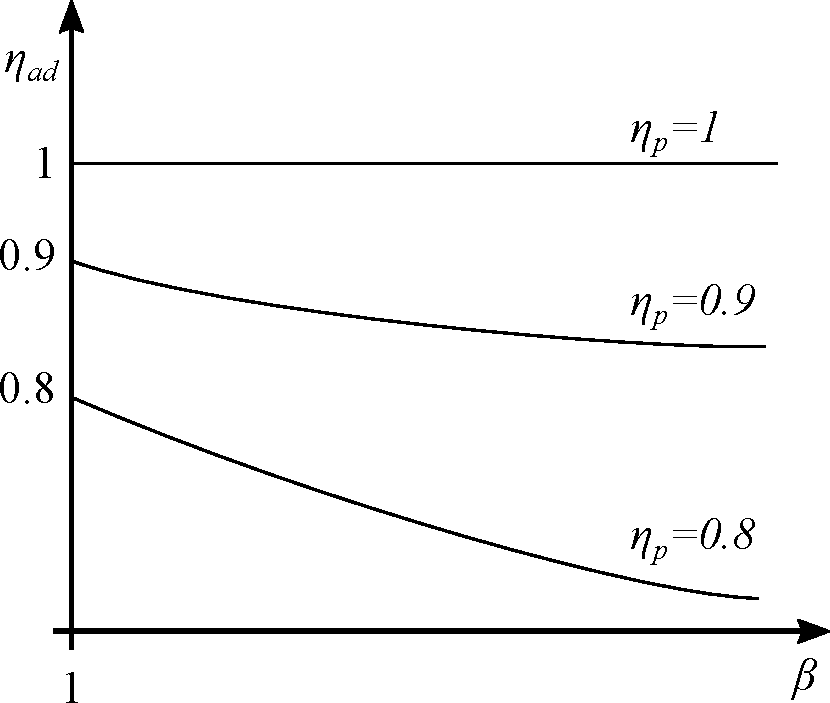
\includegraphics[width=.9\linewidth]{fig/Rend3.pdf}
  \captionof{figure}{}
  \label{fig:Rend3}
\end{minipage}%
\begin{minipage}{.55\textwidth}
  \centering
  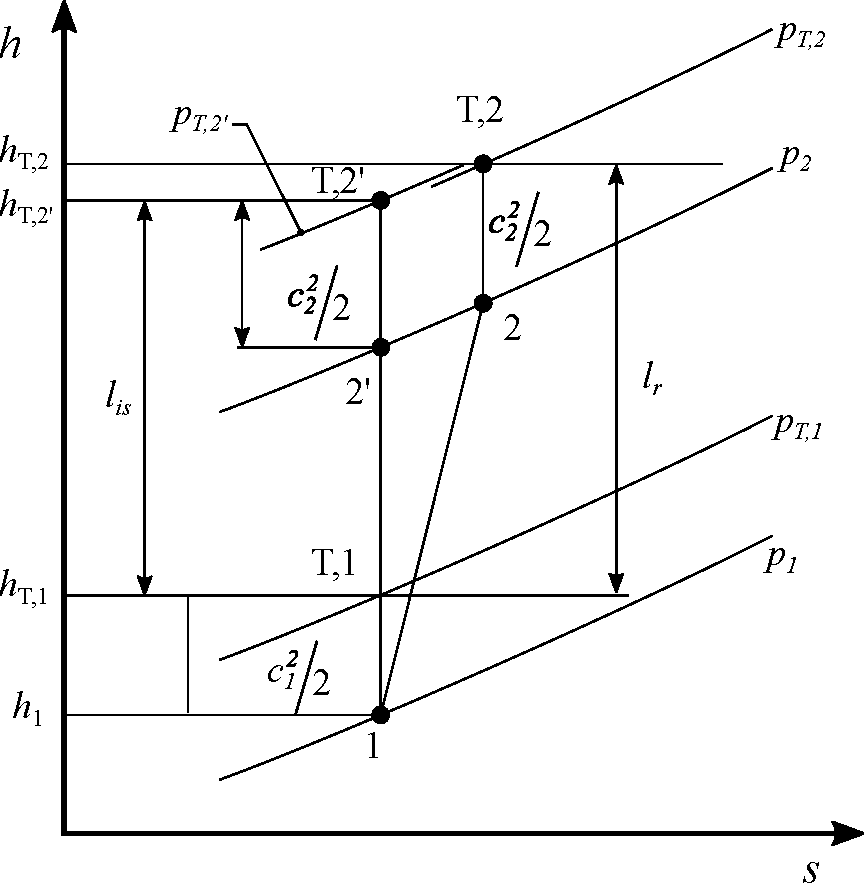
\includegraphics[width=.9\linewidth]{fig/Rend4.pdf}
  \captionof{figure}{}
  \label{fig:Rend4}
\end{minipage}
\end{figure}
Infatti poichè $\eta_p = l_p / l_r$ e $\eta_{ad} = l_{is} / l_r$, si ottiene:
\begin{align*}
\eta_{ad} = \eta_p \frac{l_{is}}{l_p} = \eta_p \frac{\left(\beta^{\frac{\gamma -1}{\gamma}}-1 \right)}{\left(\beta^{\frac{n -1}{n}}-1 \right)}
\end{align*}
ed essendo $l_p > l_{is}$ si ottiene $\eta_{ad} < \eta_p$.

Al fine di evidenziare la differenza tra le due trasformazioni è possibile definire il lavoro di controrecupero definito come:
\begin{align*}
f = \frac{l_p - l_{is}}{l_{is}} = \frac{l_p}{l_{is}} -1 = \frac{\left( \beta^{\frac{n-1}{n}} -1 \right)}{\left( \beta^{\frac{\gamma-1}{\gamma}} -1 \right)} -1 = \frac{\eta_p}{\eta_{ad}} -1
\end{align*}
Al crescere della differenza tra i due rendimenti, il fattore di controrecupero aumenta. Tale fattore è sempre maggiore di zero e si annulla quando i due rendimenti sono uguali, cioè quando non ci sono effetti termici sulla densità come avviene per le macchine idrauliche.

Qualora si vogliano studiare gli effetti delle quote cinetiche, è possibile definire diversi tipi di rendimento, sempre definiti nella scia del rendimento adiabatico, denominati "Total to Total" e "Total to Static". Con riferimento alla figura \ref{fig:Rend4} si definiscono:
\begin{itemize}
\item Rendimento Total to Total:
\begin{align*}
\eta_{T,T} = \frac{h_{T,2'} - h_{T,1}}{h_{T,2} - h_{T,1}} = \frac{h_{2'} - h_1 + \left( \frac{c_2^2 - c_1^2}{2} \right)}{h_2 - h_1 + \left( \frac{c_2^2 - c_1^2}{2} \right)} = \frac{l_{is}}{l_r}
\end{align*}
\item Rentimento Total to Static:
\begin{align*}
\eta_{T,S} = \frac{h_{2'} - h_{T,1}}{h_{T,2} - h_{T,1}} = \frac{h_{2'} - h_1 + \left( \frac{ c_1^2}{2} \right)}{h_2 - h_1 + \left( \frac{c_2^2 - c_1^2}{2} \right)} = \frac{h_{2'} - h_1 + \left( \frac{c_1^2}{2} \right)}{l_r}
\end{align*}
\end{itemize}
\pagebreak
